\documentclass[aspectratio=1610]{beamer}
\usetheme{boxes}
\usecolortheme{crane}
\usepackage{amsmath,amsfonts}
\usepackage{algpseudocode}
\usepackage{multicol}
\usepackage{pgfplots}
\pgfplotsset{compat=1.15}
\usepackage{mathrsfs}
\usetikzlibrary{arrows}
\usepackage{listings}
\lstset{
  language=Python,
  columns=flexible,
}

\usepackage{array}
\newenvironment{hashtable}[1][]
  {\begin{tabular}[#1]{
     @{}
     > {\small} r <{\normalsize~\rlap{\fbox{\strut~~}}$~~\rightarrow$~}
     @{} l @{}}}
  {\end{tabular}}



%-------------------------------------------------------------------
%	 TITLE SLIDE
%-------------------------------------------------------------------


\begin{document}

% -------------------------------------------------------------------
% Lesson 3
% -------------------------------------------------------------------
\section{Data Structures and Algorithms}

\begin{frame}
\begin{center}
\Huge Lesson 3\\~\\
\textbf{Data Structures and Algorithms DSA}
\end{center}
\end{frame}


\begin{frame}
\frametitle{Lesson 3}

\huge In this lesson we will talk about:
\begin{itemize}
	\item \alert{data structures}
	\item \alert{algorithm design}
	\item \alert{algorithm efficiency}
	\item \alert{searching and sorting algorithms}
\end{itemize}
\end{frame}


\begin{frame}{Lesson 3}{}
\begin{center}
\Huge \textbf{Data Structures}
\end{center}
\end{frame}


\begin{frame}{Lesson 3}{}
\Huge{What is a data structure?}\\~\\
\includegraphics[scale=0.80]{Images/ds}
\end{frame}


\begin{frame}{Lesson 3}{}
\LARGE
\textbf{Data Structures}\\~\\
\begin{itemize}
    \item How do we \textbf{organize} data
    \item For a very \textbf{efficient} access
\end{itemize}

It's a collection of data values, and the relationships among these values
\end{frame}


\begin{frame}{Lesson 3}{}
\LARGE
\textbf{Data Structures}
\begin{center}
\includegraphics[scale=0.80]{Images/data_structures}
\end{center}
\end{frame}



\begin{frame}
\frametitle{Lesson 3}
\LARGE 
\textbf{Linear Data Structures: Arrays, Queues, Stacks}\\~\\
\begin{itemize}
	\item Elements are arranged sequentially, one after the other
	\item The first element added will be the first one to be accessed or removed, and the last element added will be the last one to be accessed or removed
	\item Can have either fixed or dynamic sizes
	\item Offer very efficient data access
\end{itemize}
\end{frame}


\begin{frame}
\frametitle{Lesson 3}
\LARGE 
\textbf{Non-linear Data Structures: Trees, Graphs}\\~\\
\begin{itemize}
	\item Elements are arranged hierarchical
	\item We can’t traverse all the elements in a single run only
	\item There are multiple levels which we must traverse
	\item It is more difficult to implement
\end{itemize}
\end{frame}


\begin{frame}{Lesson 3}{}
\LARGE
\textbf{Data structures}
\begin{itemize}
    \item Sets
    \item Arrays and Matrices
    \item Stacks
    \item Queues
    \item Linked lists
    \item Trees
    \item Graphs
\end{itemize}
\end{frame}


\begin{frame}{Lesson 3}{}
\begin{center}
\Huge Sets
\end{center}
\end{frame}


\begin{frame}{Lesson 3}{Sets}
\LARGE
\textbf{Sets}\\~\\
A set is usually a \textbf{collection} of different things, fixed in size. Sets can also change size, usually when an algorithm will perform modifications against the set. We call these dynamic sets. These sets can change in size, grow or shrink, basically change over the time.
\end{frame}


\begin{frame}{Lesson 3}{Sets}
\Huge{But what is a set?}\\~\\
\end{frame}


\begin{frame}{Lesson 3}{Sets}
\LARGE
\textbf{Sets}\\~\\
The basic, fundamental data structure: \{1,2,4,51,9\}
\begin{itemize}
    \item mathematical set
    \item unchanging, unique elements, no duplicates
    \item contains a fixed number of elements: finite set
    \item or it can contain an infinite number of elements
\end{itemize}

\end{frame}


\begin{frame}{Lesson 3}{Sets}
\LARGE
\textbf{For example a set of polygons}
\begin{center}
\includegraphics[scale=0.10]{Images/set}
\end{center}
\end{frame}


\begin{frame}{Lesson 3}{Sets}
\LARGE
\textbf{Sets}\\~\\
A set is a \textbf{mathematical model} of a collection of different things. A set contains elements or members, which can be mathematical objects of any kind numbers, symbols, points in space, lines, other geometrical shapes, variables, or even other sets.

\end{frame}


\begin{frame}{Lesson 3}{Sets}
\LARGE
\textbf{Sets, examples}\\~\\
\begin{itemize}
    \item \{white, blue, red, yellow\}
    \item The empty set \{\}
    \item Natural numbers: $\mathbb{N} = \{0, 1, 2, 3, \ldots\}$
    \item Natural numbers except 0: $\mathbb{N^*} = \{1, 2, 3, \ldots\}$
    \item Integers: $\mathbb{Z} = \{\ldots, -3, -2, -1, 0, 1, 2, 3, \ldots\}$
    \item Positive integers: $\mathbb{Z_+} = \{0, 1, 2, 3, \ldots\}$
\end{itemize}
\end{frame}



\begin{frame}{Lesson 3}{Sets}
\LARGE{\textbf{\{1,2,3,4\}}}\\~\\
\LARGE
Defines a list of elements, using a simple enumeration notation (Roster notation) between curly brackets, separated by commas.
\end{frame}


\begin{frame}{Lesson 3}{Sets}
\LARGE
\textbf{Basic Operations on Sets}\\~\\
\begin{itemize}
    \item Insert - add a new element to a set
    \item Delete - remove an element from a set
    \item Test - if element X belongs to a set or not 
\end{itemize}

A dynamic set which supports all these basic operations: \textbf{a dictionary} 
\end{frame}


\begin{frame}{Lesson 3}{Sets}
\begin{center}
\includegraphics[scale=0.45]{Images/numbers3}
\end{center}
\end{frame}


\begin{frame}{Lesson 3}{Sets}
\begin{center}
\includegraphics[scale=0.14]{Images/NZQRC}
\end{center}
\end{frame}


\begin{frame}{Lesson 3}{Sets}
\LARGE
\textbf{Advantages}\\~\\
Perform operations on a collection of elements in a very \textbf{efficient} and \textbf{organized} manner
\end{frame}


\begin{frame}{Lesson 3}{Sets}
\LARGE
\textbf{Conclusions}\\~\\
Sets are basic, fundamental data structures, with:
\begin{itemize}
    \item unique elements
    \item no duplicates
    \item unchanging 
    \item fixed or infinite number of elements
\end{itemize}

\end{frame}


\begin{frame}{Lesson 3}{Sets}
\LARGE
\textbf{Im confused. Does it mean a set is similar to a Python set? Or what is the difference?}
\end{frame}


\begin{frame}{Lesson 3}{Sets}
\LARGE
\textbf{Sets vs. Python Set}\\~\\
In computer science (CS), a set is an abstract data type that can store unique values, without any particular order. It is a computer implementation of the mathematical concept of a finite set.
\end{frame}



\begin{frame}{Lesson 3}{Sets}
\LARGE
\textbf{Mathematical vs. Python Sets}\\~\\
\begin{itemize}
    \item Mathematical finite set: \{1,2,3,4\}
    \item Python set: S = \{1,2,3,4\}
\end{itemize}
\end{frame}



% %%%%%%%%%%%%%%%%%%%%%%%%%%%%%%%%%%%%%%%%%%%%%%%%%%%%
% Arrays
% %%%%%%%%%%%%%%%%%%%%%%%%%%%%%%%%%%%%%%%%%%%%%%%%%%%%

\begin{frame}{Lesson 3}{}
\begin{center}
\Huge Arrays
\end{center}
\end{frame}

\begin{frame}{Lesson 3}{Arrays}
\LARGE
\textbf{Arrays}\\~\\
In computer science, an \textbf{array} is a data structure consisting of a collection of elements, each identified by an \textbf{index} or a \textbf{key}. The simplest type of such data structure is a linear array, the one-dimensional array.
\end{frame}


\begin{frame}{Lesson 3}{Arrays}
\begin{center}
\includegraphics[scale=0.17]{Images/array2.png}
\end{center}
\end{frame}



\begin{frame}{Lesson 3}{Arrays}
\LARGE
\textbf{Arrays}\\~\\
Arrays are among the oldest and most important data structures, and are used by almost every program and programming language. They are also used to implement many other data structures, such as lists.
\end{frame}


\begin{frame}{Lesson 3}{Arrays}
\LARGE
\textbf{Arrays}\\~\\
Arrays are useful because the element indices can be computed at \alert{run time}. Among
other things, this feature allows a single iterative statement to process arbitrarily many
elements of an array. For that reason, the elements of an array data structure are required
to have the same size and should use the same data representation. 
\end{frame}



\begin{frame}{Lesson 3}{Arrays}
\LARGE
\textbf{Run-time?}\\~\\
Runtime, run time, or execution time is the final phase of a computer program's life cycle,
in which the code is being executed on the computer's central processing unit (CPU) as
machine code. In other words, "runtime" is the running phase of a program.
\end{frame}



\begin{frame}{Lesson 3}{Arrays}
\Large
\textbf{Remember this? From source code to executable}\\~\\ 
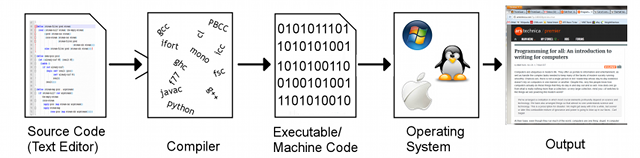
\includegraphics[scale=0.65]{Images/CompilationChain}
\end{frame}



\begin{frame}{Lesson 3}{}
\LARGE
\textbf{Basic Array Operations}\\~\\
\begin{itemize}
	\item traversal of an array
	\item access element X in an array
	\item searching element X in an array
	\item sorting an array
\end{itemize}
\end{frame}



\begin{frame}{Lesson 3}{Arrays}
\Large
\textbf{Example 1: Traversing the array A}\\~\\

\label{getArray}
\begin{algorithmic}[1]
\Procedure{getArray}{$A$} \Comment{Returns the max value in A}
\State $L\gets length(A)$
\For{\texttt{i=0 to L-1}}
    \State print $A[i]$
\EndFor
\EndProcedure
\end{algorithmic}
\end{frame}


\begin{frame}[fragile]
\LARGE
\textbf{Traversing the array}\\~\\
\Large
\begin{lstlisting}
A = [1, 2, 3, 4, 5, 6, 7,8,9]

# Traversing the array
for element in A:
    print(element, end=" ")}
\end{lstlisting}
\end{frame}



\begin{frame}[fragile]
\LARGE
\textbf{Traversing the array, version 2}\\~\\
\Large
\begin{lstlisting}
A = [1, 2, 3, 4, 5, 6, 7,8,9]

# Traversing the array
for i in range(len(A)):
    print(A[i], end=" ")
\end{lstlisting}
\end{frame}




\begin{frame}{Lesson 3}{Arrays}
\Large
\textbf{Example 2: Find the max value in the array A}\\~\\

\label{MaxArray}
\begin{algorithmic}[1]
\Procedure{MaxArray}{$A$} \Comment{Returns the max value in A}
\State $N\gets length(A)$
\State $MAX\gets A[0]$
\For{\texttt{from i=1 to N-1}}
\If {$A[i] > MAX$}
    \State \textbf{$MAX = A[i]$} \Comment{The MAX is A[i]}
\EndIf
\EndFor
\State \Return $MAX$
\EndProcedure
\end{algorithmic}
\end{frame}



\begin{frame}{Lesson 3}{Arrays}
\Large
\textbf{Example 3: Search element X in array A}\\~\\
\label{SearchArray}
\begin{algorithmic}[1]
\Procedure{SearchArray}{$A$} \Comment{Returns the max value in A}
\State $X\gets MyElement$
\State $N\gets length(A)$
\For{\texttt{from i=0 to N-1}}
\If {$X = A[i]$}
    \State \Return {$i$}  \Comment{The index for my match}
\EndIf
\EndFor
\State \Return -1 \Comment{otherwise return -1}
\EndProcedure
\end{algorithmic}
\end{frame}



\begin{frame}[fragile]
\LARGE
\textbf{Search element in array}\\~\\
\Large
\begin{lstlisting}[language=Python]
A = [1, 2, 3, 4, 5, 6, 7,8,9]

def find_element(A, n, key):
    for i in range(n):
        if A[i] == key:
            return i
    return -1

\end{lstlisting}
\end{frame}




\begin{frame}{Lesson 3}{}
\LARGE
\textbf{There are numerous applications of arrays}\\
\begin{itemize}
    \item Storing data in databases. Storing a list of customer names.  
    \item Traffic Management.Traffic management systems use arrays to track vehicles and
    their flow. By analyzing data stored in arrays, traffic control centers can implement
    efficient signal timings and manage congestion effectively.
\end{itemize}
\end{frame}



\begin{frame}{Lesson 3}{Arrays}
\LARGE
\begin{itemize}
    \item Financial Analysis. It keeps track of various financial instruments, including stocks, bonds, and mutual funds. By organizing data in arrays, companies can perform analyses and make predictions easier 
    \item Machine Learning. Machine learning algorithms often accept arrays as input, helping to train models and make predictions.
\end{itemize}
\end{frame}



% %%%%%%%%%%%%%%%%%%%%%%%%%%%%%%%%%%%%%%%%%%%%%%%%%%%%
% Matrices
% %%%%%%%%%%%%%%%%%%%%%%%%%%%%%%%%%%%%%%%%%%%%%%%%%%%%
\begin{frame}{Lesson 3}{Matrices}
\begin{center}
\Huge Matrices
\end{center}
\end{frame}


\begin{frame}{Lesson 3}{Matrices}
\LARGE
\textbf{What is a matrix?}\\~\\
In mathematics, a matrix (pl.: matrices) is a rectangular array or table of numbers,
symbols, or expressions, with elements or entries arranged in rows and columns, which is
used to represent a mathematical object or property of such an object.
\end{frame}


\begin{frame}{Lesson 3}{Matrices}
\LARGE
\textbf{Matrices}
\begin{center}
\includegraphics[scale=0.14]{Images/matrices2}
\end{center}
\end{frame}


\begin{frame}{Lesson 3}{Matrices}
\LARGE
\textbf{Matrices}
\begin{center}
\includegraphics[scale=0.10]{Images/Matrix}
\end{center}
\end{frame}


\begin{frame}[fragile]
\LARGE
\textbf{Matrix multiplication}\\~\\
   \[  \begin{bmatrix}
         0 & 1\\ 
         0 & 0 
     \end{bmatrix}
     \times
     \begin{bmatrix}
         0 & 0\\ 
         1 & 0  
     \end{bmatrix}
      =
     \begin{bmatrix}
         1 & 0\\ 
         0 & 0   
     \end{bmatrix} \] 
\end{frame}


\begin{frame}[fragile]
\LARGE
\textbf{Matrix multiplication M x N}\\~\\
\Large
    \[ \begin{bmatrix}
         a_{11} & a_{12} & \cdots & a_{1n}\\
         a_{21} & a_{22} & \cdots & a_{2n}\\ 
         \vdots & \vdots & \ddots & \vdots\\ 
         a_{m1} & a_{m2} & \cdots & a_{mn} 
     \end{bmatrix}
     \times
     \begin{bmatrix}
         b_{11} & b_{12} & \cdots & b_{1p}\\
         b_{21} & b_{22} & \cdots & b_{2p}\\ 
         \vdots & \vdots & \ddots & \vdots\\ 
         b_{n1} & b_{n2} & \cdots & b_{np} 
     \end{bmatrix}
      =
     \begin{bmatrix}
         c_{11} & c_{12} & \cdots & c_{1p}\\
         c_{21} & c_{22} & \cdots & c_{2p}\\ 
         \vdots & \vdots & \ddots & \vdots\\ 
         c_{m1} & c_{m2} & \cdots & c_{mp} 
     \end{bmatrix} \]
  \[ c_{ij}= a_{i1} b_{1j} + a_{i2} b_{2j} +\cdots+ a_{in} + b_{nj} = \sum_{k=1}^n a_{ik}b_{kj} \]
\end{frame}


\begin{frame}{Lesson 3}{Matrices}
\LARGE
\textbf{Basic Matrix Operations}\\~\\
\begin{itemize}
	\item access X element in a matrix
	\item traversal of a matrix
	\item searching a matrix
	\item sorting a matrix
\end{itemize}
\end{frame}




\begin{frame}[fragile]
\LARGE
\textbf{Accessing the elements of a matrix}\\~\\
\Large
\begin{lstlisting}[language=Python]
A = [[1, 2, 3], [4, 5, 6], [7,8,9]]

# Accessing certain elements in a matrix
print("1st element of 1st row:", A[0][0])
print("2nd element of the 2nd row:", A[1][2])
print("2nd element of 3rd row:", A[2][1])
\end{lstlisting}
\end{frame}



\begin{frame}[fragile]
\LARGE
\textbf{Traversing the matrix}\\~\\
\Large
\begin{lstlisting}[language=Python]
A = [[1, 2, 3], [4, 5, 6], [7,8,9]]

# Traversing the matrix
for row in A:
    # Traversing the matrix
    for x in row:
        print(x, end=" ")
    print()
\end{lstlisting}
\end{frame}



\begin{frame}{Lesson 3}{Matrices}
\LARGE
\textbf{There are numerous applications of matrices}\\
\begin{itemize}
    \item Encryption: Matrices encrypt data into unreadable formats and decode it for secure communication. 
    \item Computer Graphics: transformations like scaling, rotation, and translation of objects in 2D and 3D graphics
    \item Machine Learning: fundamental data structures for neural networks  
\end{itemize}
\end{frame}


\begin{frame}{Lesson 3}{Matrices}
\LARGE
\begin{itemize}
	\item Economics and Business: optimize business operations like supply chains and financial forecasting
	\item Navigation Systems: GPS systems use matrices to calculate positions, distances, and directions in 2D and 3D space.
	\item Weather Prediction: Matrices solve systems of differential equations to model and predict climate and weather patterns
\end{itemize}
\end{frame}


% %%%%%%%%%%%%%%%%%%%%%%%%%%%%%%%%%%%%%%%%%%%%%%%%%%%%
% Stacks
% %%%%%%%%%%%%%%%%%%%%%%%%%%%%%%%%%%%%%%%%%%%%%%%%%%%%
\begin{frame}{Lesson 3}{Stacks}
\begin{center}
\Huge Stacks
\end{center}
\end{frame}


\begin{frame}{Lesson 3}{Sets}
\Huge{What is a stack?}\\~\\
\end{frame}

\begin{frame}{Lesson 3}{Stacks}
\LARGE
The stack is an analogy to a set of physical items stacked one atop
another, such as a stack of plates.
\end{frame}

\begin{frame}{Lesson 3}{Stacks}
\begin{center}
\includegraphics[scale=0.23]{Images/stack}
\end{center}
\end{frame}


\begin{frame}{Lesson 3}{Stacks}
\LARGE
\textbf{Stacks}\\~\\
Stacks are collections of elements, which support two main operations:\\
\begin{itemize}
    \item \textbf{PUSH}: which adds an element to the collection 
    \item \textbf{POP}: which removes the most recent elements from the collection
\end{itemize}
\end{frame}


\begin{frame}{Lesson 3}{Stacks}
\LARGE
\textbf{Stacks}\\~\\
There might be, another operation called \textbf{PEEK}, which without
modifying the stack, return the value of the last element added.
\end{frame}


\begin{frame}{Lesson 3}{Stacks}
\LARGE
\textbf{Stacks}\\~\\
\begin{itemize}
    \item \textbf{PUSH}: which adds an element to the collection 
    \item \textbf{POP}: which removes the most recent elements from the collection
    \item \textbf{PEEK}: returns the value of the last element added
\end{itemize}
\end{frame}


\begin{frame}{Lesson 3}{Stacks}
\LARGE
\textbf{Stacks}\\~\\
The stack supports few operations. And it operates in a certain,
predefined order. The order in which an element added to or removed
from a stack is described as last in, first out,
referred to by the acronym \textbf{LIFO}
\end{frame}


\begin{frame}{Lesson 3}{Stacks}
\begin{center}
\includegraphics[scale=0.13]{Images/Lifo_stack}
\end{center}
\end{frame}


\begin{frame}{Lesson 3}{Stacks}
\LARGE
\textbf{Stacks}\\~\\
"Stacks entered the computer science literature in 1946, when
\alert{Alan Turing} used the terms "bury" and "unbury" as a means of
calling and returning from subroutines."
\end{frame}



\begin{frame}{Lesson 3}{Stacks}
\Huge 
\textbf{Stacks}\\~\\
How can we implement a stack? 
\end{frame}


\begin{frame}{Lesson 3}{Stacks}
\LARGE
\textbf{Stacks}\\~\\
A stack can be easily implemented using an array. The first
element, usually at the zero offset, is the bottom, resulting in
array[0] being the first element pushed onto the stack and the last
element popped off. 
\end{frame}

\begin{frame}{Lesson 3}{Stacks}
\LARGE
\textbf{Stacks}\\~\\
The program must keep track of the size (length) of the stack, using a variable 
top that records the number of items pushed so far, therefore pointing to the 
place in the array where the next element is to be inserted (assuming a zero-based 
index convention).
\end{frame}



\begin{frame}{Lesson 3}{Stacks}
\LARGE
\textbf{Stacks}\\~\\
The program must keep track of the size (length) of the stack, using
a variable top that records the number of items pushed so far,
therefore pointing to the place in the array where the next element
is to be inserted (assuming a zero-based index convention).
\end{frame}


\begin{frame}[fragile]
\Large
\textbf{Stack using arrays}\\~\\
\begin{lstlisting}[language=Python]

# Create a stack. It initializes size of stack as 0 
def createStack(): 
    stack = [] 
    return stack 
\end{lstlisting}
\end{frame}

\begin{frame}[fragile]
\Large
\begin{lstlisting}[language=Python]
# Stack is empty when stack size is 0 
def isEmpty(stack): 
    return len(stack) == 0

# Add an item to stack. It increases size by 1 
def push(stack, item): 
    stack.append(item) 
    print(item + " pushed to stack ")
 \end{lstlisting}
\end{frame} 
    
    
\begin{frame}[fragile]
\Large
\begin{lstlisting}[language=Python]    
# Remove an item from stack. It decreases size by 1 
def pop(stack): 
    if (isEmpty(stack)): 
        # return minus infinite
        return str(-maxsize -1) 
    return stack.pop() 

# Return the top from stack without removing it 
def peek(stack): 
    if (isEmpty(stack)): 
        # return minus infinite
        return str(-maxsize -1)  
    return stack[len(stack) - 1] 
 \end{lstlisting}
\end{frame}


\begin{frame}[fragile]
\LARGE
\textbf{Stack using LiFoQueue}\\~\\
\Large
\begin{lstlisting}[language=Python]
from queue import LifoQueue
stack = LifoQueue()
stack.put(1)
stack.put(2)
stack.put(3)
print(stack.get()) # Prints 3
print(stack.get()) # Prints 2
\end{lstlisting}
\end{frame}



\begin{frame}{Lesson 3}{Stacks}
\LARGE
\textbf{There are numerous applications of stacks}\\
\begin{itemize}
    \item Undo mechanism in text editors
    \item Fwd and back buttons on web browsers
    \item Memory management in computer programming (static memory allocation. It can be used to keep track of functions calls)
    \item Implementing \alert{recursion}
\end{itemize}
\end{frame}



\begin{frame}{Lesson 3}{Stacks}
\Huge
 But what is recursion?
\end{frame}


\begin{frame}{Lesson 3}{Stacks}
\LARGE
\textbf{Recursion}\\
\begin{itemize}
    \item It is a programming technique, a way to program and develop a program where a function calls itself many times
    \item You take a big problem, into smaller problems, trying to apply a solution to solve the small problems
    \item You define a problem in terms of itself 
\end{itemize}
\end{frame}


\begin{frame}{Lesson 3}{Stacks}
\LARGE
\textbf{Recursion}\\~\\
You are standing in a long queue of people. You must answer, how many
people are behind you in the line?\\~\\
\large
\textbf{Note:}
One person can see only the person standing directly in front and
behind. One cannot look back and count. Each person is allowed to ask
questions from the person standing in front or behind.
\end{frame}


\begin{frame}{Lesson 3}{Stacks}
\LARGE
\textbf{Recursion}\\~\\
You look behind and see if there is a person there. If not, then you
can return the answer "0". If there is a person, repeat this step 
and wait for a response from the person standing behind. Once a
person receives a response, they add 1 and respond to the person
that asked them or the person standing in front of them.
\end{frame}


\begin{frame}{Lesson 3}{Stacks}
\Large
\textbf{Recursion example}\\~\\
\label{personCount}
\begin{algorithmic}[1]
\Procedure{personCount}{$currPerson$}
\If {$noOneBehind(currPerson) == TRUE$}
    \State \Return {$0$}
\Else { $personBehind == currPerson.checkBehind$ }
    \State \Return {$1 + \Call{personCount}{$}}    
\EndIf
\EndProcedure
\end{algorithmic}
\end{frame}



\begin{frame}{Lesson 3}{Stacks}
{\LARGE\textbf{{Thinking recursively}}}
\Large
\begin{minipage}{0.60\textwidth}
    \begin{itemize}
      \item Learning to look for big things 
      \item That are made from smaller things
    \end{itemize}
  \end{minipage}
\begin{minipage}{.0\textwidth}
    % Show the image at item three and afterwards
      \begin{figure}
        \includegraphics[scale=0.30]{Images/recursion}
      \end{figure}
  \end{minipage}  
\end{frame}



\begin{frame}{Lesson 3}{Stacks}
\LARGE
\textbf{Solving a problem recursively}\\~\\
\underline{Recursion is a function calling itself} until a generic,
base condition is true to produce the correct output. In other 
words, to solve a problem, we solve a problem that is a smaller
instance of the same problem, and then use the solution to that
smaller instance to solve the original problem.
\end{frame}



\begin{frame}{Lesson 3}{Stacks}
\LARGE
\textbf{Factorial number}\\~\\
In mathematics, the factorial of a non-negative integer 
$n!$ is the product of all positive integers less than or equal to n
\begin{equation}
n!=n \times (n-1)!
\end{equation}
\begin{equation}
n! = n \times (n-1) \times (n-2) \times \dots 3 \times 2 \times 1
\end{equation}
\end{frame}


\begin{frame}{Lesson 3}{Stacks}
\begin{center}
\includegraphics[scale=0.99]{Images/factorial2}
\end{center}
\end{frame}



\begin{frame}{Lesson 3}{Stacks}
\begin{center}
\includegraphics[scale=0.55]{Images/factorial1}
\includegraphics[scale=0.55]{Images/factorial11}
\end{center}
\end{frame}



\begin{frame}{Lesson 3}{Stacks}
\Large
\textbf{Recursion example}\\~\\
\label{factorial}
\begin{algorithmic}[1]
\Procedure{factorial}{$N$}
\If {$N == 0$}
    \State \Return {$1$}
\Else
    \State \Return {$N * \Call{factorial}{N-1}$}
\EndIf
\EndProcedure
\end{algorithmic}
\end{frame}


\begin{frame}[fragile]
\Large
\textbf{Factorial, using recursion}\\~\\
\begin{lstlisting}[language=Python]

def factorial(n):
    if n == 1:
        return 1
    else:
        return n * factorial(n-1)

print(factorial(5))
 \end{lstlisting}
\end{frame} 


\begin{frame}{Lesson 3}{Stacks}
\LARGE
\textbf{Solving a problem recursively}\\~\\
For a recursive algorithm to work, smaller subproblems must
be found and arrive at the base case. In simple words, any recursive
algorithm has two parts: the base case and the recursive structure.
\end{frame}


\begin{frame}{Lesson 3}{Stacks}
\LARGE
\textbf{The Base Case}\\~\\
The base case is a terminating condition where a function
immediately returns the result. This is the smallest version of the
problem for which we already know the solution.
\end{frame}

\begin{frame}{Lesson 3}{Stacks}
\LARGE
\textbf{The Recursive structure}\\~\\
The recursive structure is an idea to design a solution to a problem
via the solution of its smaller sub-problems, i.e., the same problem
but for a smaller input size. We continue calling the same problem
for smaller input sizes until we reach the base case of recursion.
\end{frame}



\begin{frame}{Lesson 3}{Stacks}
\LARGE
\textbf{How recursion works?}\\~\\

If we draw the flow of recursion for the factorial program, one can
find this pattern: we are calling fact(0) last, but it is returning
the value first. Similarly, we are calling fact(n) first, but it is
returning the value last. Its a Last In First Out (LIFO) order for
all recursive calls and return values.
\end{frame}



\begin{frame}{Lesson 3}{Stacks}
\LARGE
\textbf{Recursion uses Stacks behind}\\~\\
Order of recursive calls: larger problem to smaller problem
$fact(n) \rightarrow fact(n -1) \rightarrow ... 	\rightarrow fact(1) 	\rightarrow fact(0)$\\~\\
Order of return values: smaller problem to larger problem
$fact(0) \rightarrow fact(1) \rightarrow ... \rightarrow fact(n - 1) \rightarrow fact(n)$
\end{frame}


\begin{frame}{Lesson 3}{Stacks}
\LARGE
\begin{minipage}{0.50\textwidth}
    Execution call stack!
  \end{minipage}
\begin{minipage}{.0\textwidth}
    % Show the image at item three and afterwards
      \begin{figure}
        \includegraphics[scale=0.40]{Images/callstack}
      \end{figure}
  \end{minipage}  
\end{frame}



\begin{frame}{Lesson 3}{Stacks}
\LARGE
\textbf{Recursion is important!}\\
\begin{itemize}
    \item the basis for Dynamic Programming and Divide and Conquer algorithms
    \item helps in solving complex problems by breaking them into smaller subproblems
    \item fundamental to sorting, like quicksort, mergesort
    \item used in traversing trees and other complex data structures
\end{itemize}
\end{frame}



\begin{frame}{Lesson 3}{Stacks}
\Huge
Recursion vs Iteration?
\end{frame}


\begin{frame}{Lesson 3}{Stacks}
\huge
A program is called \textbf{recursive} when an entity calls itself.
A program is called \textbf{iterative} when there is a loop (or
repetition) of some sort.
\end{frame}



\begin{frame}{Lesson 3}{Stacks}
\LARGE
\textbf{Recursion}\\
\begin{minipage}{0.53\textwidth}
\begin{itemize}
    \item each function call creates a smaller problem to solve
    \item and these calls continue until reaching a basic case which is trivial to solve
\end{itemize}
  \end{minipage}
\begin{minipage}{.0\textwidth}
    % Show the image at item three and afterwards
      \begin{figure}
        \includegraphics[scale=0.30]{Images/recursion_effect}
      \end{figure}
  \end{minipage}  
\end{frame}



\begin{frame}{Lesson 3}{Stacks}
\LARGE
\textbf{Recursive function}\\
\begin{minipage}{0.60\textwidth}
\Large
\begin{itemize}
    \item \textbf{Base case} The condition under which the function stops calling itself. This prevents infinite recursion and provides a direct answer for the simplest instance of the problem.
    \item \textbf{Recursive case} The part of the function that reduces the problem into smaller instances and calls itself with small data.
\end{itemize}
  \end{minipage}
\begin{minipage}{.0\textwidth}
    % Show the image at item three and afterwards
      \begin{figure}
        \includegraphics[scale=0.26]{Images/recursion_flowchart}
      \end{figure}
  \end{minipage}  
\end{frame}



\begin{frame}[fragile]
\Large
\textbf{Recursive Factorial}\\~\\
\begin{lstlisting}
def factorial(n):
    # Base case: if n is 1 or 0, factorial is 1
    if n == 0 or n == 1:
        return 1
    # Recursive case: n * factorial of (n-1)
    else:
        return n * factorial(n - 1)
print(factorial(5))
 \end{lstlisting}
\end{frame}


\begin{frame}{Lesson 3}{Stacks}
\LARGE
\textbf{Recursion Types}\\
\begin{itemize}
    \item direct recursion
    \item indirect recursion
    \item tail recursion 
\end{itemize}
\end{frame}



\begin{frame}[fragile]
\Large
\textbf{Direct Recursion} - the simplest form of recursion. A function directly calls itself within its definition. \\~\\
\begin{lstlisting}[language=Python]
def direct_recursion(n):
    if n <= 0:
        return
    print(n)
    direct_recursion(n - 1)
 \end{lstlisting}
\end{frame} 



\begin{frame}[fragile]
\Large
\textbf{Indirect Recursion} - creates a cylces of function calls. A function calls another function, which calls the original function.\\~\\
\begin{lstlisting}[language=Python]
def functionA(n):
    if n <= 0:
        return
    print(n)
    functionB(n - 1)

def functionB(n):
    if n <= 0:
        return
    print(n)
    functionA(n - 2)
 \end{lstlisting}
\end{frame} 

    
\begin{frame}[fragile]
\Large
\textbf{Tail Recursion} - the recursive call is the last operation in the function.\\~\\
\begin{lstlisting}[language=Python]
def tail_recursion(n, aggregate=1):
    if n == 0:
        return aggregate
    return tail_recursion(n - 1, n * aggregate)
 \end{lstlisting}
\end{frame} 



\begin{frame}{Lesson 3}{Stacks}
\LARGE
\textbf{Iterative}\\
\begin{minipage}{0.60\textwidth}
\begin{itemize}
    \item a repetitive process
    \item runs a number of times until a specified condition is met
    \item or certain number of iterations have been reached
\end{itemize}
  \end{minipage}
\begin{minipage}{.0\textwidth}
    % Show the image at item three and afterwards
      \begin{figure}
        \includegraphics[scale=0.30]{Images/iteration}
      \end{figure}
  \end{minipage}  
\end{frame}



\begin{frame}{Lesson 3}{Stacks}
\LARGE
\textbf{Iterative function}\\
\begin{minipage}{0.60\textwidth}
\Large
\begin{itemize}
    \item \textbf{Initialization} Start with initializing variables or setting initial conditions required for the iterative process
    \item \textbf{Condition} Check a condition that determines whether the iteration should continue or stop
    \item \textbf{Body} Execute a set of instructions or operations that represent the core logic of the iteration. 
\end{itemize}
  \end{minipage}
\begin{minipage}{.0\textwidth}
    % Show the image at item three and afterwards
      \begin{figure}
        \includegraphics[scale=0.30]{Images/iterative_flowchart}
      \end{figure}
  \end{minipage}  
\end{frame}



\begin{frame}{Lesson 3}{Stacks}
\LARGE
\textbf{How to build an iterative function?}\\
\begin{itemize}
    \item loops: while, do-while, for loops
    \item for loop: when the number of iterations is known beforehand
    \item while loop: when the number of iterations is unknown, and the loop continues as long as a condition is true
    \item do-while loop: same as while loop but ensures that the loop is executed at least once before the condition is tested
\end{itemize}
\end{frame}



\begin{frame}[fragile]
\LARGE
\textbf{Iterative Factorial} - the iterative function to calculate the factorial\\
\Large
\begin{lstlisting}[language=Python]
def factorial(n):
    result = 1
    for i in range(1, n + 1):
        result *= i
    return result
print(factorial(5))
 \end{lstlisting}
\end{frame}



\begin{frame}{Lesson 3}{Stacks}
\LARGE
\textbf{When to use recursion vs. iteration}\\
The nature of the problem
\begin{itemize}
    \item naturally fit a recursive structure or require breaking down into smaller subproblems
    \item for loop: when the number of iterations is known beforehand
    \item use iteration for problems with a straightforward repetitive process or when the number of iterations is known beforehand
\end{itemize}
\end{frame}


\begin{frame}{Lesson 3}{Stacks}
\LARGE
\textbf{When to use recursion vs. iteration}\\
Complexity and readability
\begin{itemize}
    \item Use recursion when it simplifies the code and makes it more readable
    \item Use iteration when recursion would make the code unnecessarily complex or when avoiding the risk of stack overflow is essential
\end{itemize}
\end{frame}



\begin{frame}{Lesson 3}{Stacks}
\LARGE
\textbf{When to use recursion vs. iteration}\\
Performance consideration
\begin{itemize}
    \item Use recursion if the problem’s recursive nature allows for more elegant and maintainable code and manageable stack usage
    \item Use iteration if memory usage is a concern and the problem can be solved efficiently with loops.
\end{itemize}
\end{frame}


\begin{frame}{Lesson 3}{Stacks}
\LARGE
\textbf{Use recursion}\\
\Large
\begin{itemize}
    \item \textbf{Divide and conquer} problems like merge sort, quicksort, and binary search where the problem is divided into smaller subproblems that are solved recursively 
    \item \textbf{Tree and graph problems} Traversals (e.g., in-order, pre-order, post-order for trees) and pathfinding in graphs that naturally fit a recursive approach.
    \item \textbf{Dynamic programming} Problems like the Fibonacci sequence, where recursion with memoization simplifies the solution
    \item \textbf{Combinatorial problems} Generating permutations and combinations and solving puzzles like the Tower of Hanoi
\end{itemize}
\end{frame}



\begin{frame}{Lesson 3}{Stacks}
\LARGE
\textbf{Use iteration}\\
\Large
\begin{itemize}
    \item \textbf{Simple loops} Problems like summing a list of numbers, iterating through arrays or lists, and simple counting problems
    \item \textbf{Linear problems} Iterative solutions for problems requiring a linear scan, such as finding an array’s maximum or minimum value
    \item  \textbf{Repetitive tasks} Problems that require repeating a task a known number of times, such as printing numbers from 1 to N or iterating through data structures like arrays and linked lists.
\end{itemize}
\end{frame}


\begin{frame}{Lesson 3}{Stacks}
\begin{center}
\includegraphics[scale=0.12]{Images/Fibonacci_Spiral}
\end{center}
\end{frame}



\begin{frame}{Lesson 3}{Stacks}
\Huge 
\textbf{Fibonacci sequence}
\end{frame}


\begin{frame}{Lesson 3}{Stacks}
\LARGE
\textbf{Fibonacci sequence}\\~\\
\begin{center}
\includegraphics[scale=0.60]{Images/Fib1}
\end{center}
\end{frame}


\begin{frame}{Lesson 3}{Stacks}
\LARGE
\textbf{Fibonacci sequence}
\begin{center}
\includegraphics[scale=0.45]{Images/Fib2}
\end{center}
\end{frame}


\begin{frame}[fragile]
\Large
\textbf{Fibonacci Recursion}\\~\\
\begin{lstlisting}[language=Python]
def fibonacci_recursive(n):
    if n <= 0:
        return 0
    elif n == 1:
        return 1
    else:
        return fibonacci_recursive(n-1) + fibonacci_recursive(n-2)

# Main Code
n = 10
print(f"Recursive method: Fibonacci({n}) = {fibonacci_recursive(n)}")
 \end{lstlisting}
\end{frame} 



\begin{frame}[fragile]
\Large
\textbf{Fibonacci Iterative}\\~\\
\begin{lstlisting}[language=Python]
def fibonacci_iterative(n):
    if n <= 0:
        return 0
    elif n == 1:
        return 1
    a, b = 0, 1
    for _ in range(2, n + 1):
        a, b = b, a + b
    return b

# Main code
n = 10
print(f"Iterative method: Fibonacci({n}) = {fibonacci_iterative(n)}")
 \end{lstlisting}
\end{frame} 



\begin{frame}{Lesson 3}{Stacks}
\LARGE
\textbf{Advantages of Stacks}\\
\Large
\begin{itemize}
\item Simplicity: Stacks are a simple and easy-to-understand data structure
\item Efficiency: Push and pop operations on a stack are very fast, providing efficient access to data.
\item LIFO: Stacks follow the LIFO principle, ensuring that the last element added to the stack is the first one removed.
\item Limited memory usage: Stacks only need to store the elements that have been pushed onto them, making them memory-efficient compared to other data structures.
\end{itemize}
\end{frame}



\begin{frame}{Lesson 3}{Stacks}
\LARGE
\textbf{Disadvantages of Stacks}\\
\Large
\begin{itemize}
\item Limited access: Elements can only be accessed from the top, making it difficult to retrieve or modify elements in the middle of the stack.
\item Overflow: If more elements are pushed onto a stack than it can hold, an overflow error will occur, resulting in a loss of data.
\item No random access: Stacks do not allow for random access to elements, making them unsuitable for applications where elements need to be accessed in a specific order.
\item Limited capacity: Fixed capacity, a limitation if the number of elements that need to be stored is unknown or highly variable.
\end{itemize}
\end{frame}



% %%%%%%%%%%%%%%%%%%%%%%%%%%%%%%%%%%%%%%%%%%%%%%%%%%%%
% Queues
% %%%%%%%%%%%%%%%%%%%%%%%%%%%%%%%%%%%%%%%%%%%%%%%%%%%%
\begin{frame}{Lesson 3}{Queues}
\begin{center}
\Huge Queues
\end{center}
\end{frame}


\begin{frame}{Lesson 3}{Queues}
\LARGE
\textbf{Queues}\\~\\
A queue is a collection of entities that are maintained in
a sequence and can be modified by the addition of entities at one
end of the sequence and the removal of entities from the other end
of the sequence. 
\end{frame}


\begin{frame}{Lesson 3}{Queues}
\begin{center}
\includegraphics[scale=0.10]{Images/Queue}
\end{center}
\end{frame}


\begin{frame}{Lesson 3}{Queues}
\LARGE
By convention, the end of the sequence at which elements are added
is called \textbf{the back, tail, or rear} of the queue, and the end
at which elements are removed is called the \textbf{head or front}
of the queue, analogously to the words used when people line up to
wait for goods or services.
\end{frame}



\begin{frame}{Lesson 3}{Queues}
\LARGE
\textbf{Queues}\\~\\
The operations of a queue make it a first-in-first-out \textbf{FIFO}
data structure. In a FIFO data structure, the first element added to
the queue will be the first one to be removed.\\
A queue is an example of a linear data structure, or more abstractly
a sequential collection.
\end{frame}


\begin{frame}{Lesson 3}{Queues}
\LARGE
\textbf{Queue Properties}\\~\\
\Large
\begin{itemize}
\item \textbf{Front:} Position of the entry in a queue ready to be served, that is, the first entry that will be removed from the queue, is called the front of the queue (head of the queue)
\item \textbf{Rear:} Position of the last entry in the queue, that is, the one most recently added, is called the rear of the queue. (tail of the queue)
\item \textbf{Size:} the current number of elements in the queue 
\item \textbf{Capacity:} the maximum number of elements the queue can hold
\end{itemize}
\end{frame}


\begin{frame}{Lesson 3}{Queues}
\LARGE
\textbf{Queue Operations}\\~\\
\Large
\begin{itemize}
\item \textbf{Enqueue} — Add an element to the end of the queue
\item \textbf{Dequeue} — Remove an element from the front of the queue
\item \textbf{Is Empty} — Check if the queue is empty
\item \textbf{Is Full} — Check if the queue is full
\item \textbf{Peek} — Get the value of the front element without removing it
\end{itemize}
\end{frame}




\begin{frame}[fragile]
\Large
\textbf{Queue implements a basic FIFO queue}\\~\\
\begin{lstlisting}[language=Python]
from queue import Queue
q = Queue()
q.put(1) # Add 1 to queue
q.put(2)
q.put(3)
print(q.qsize()) # Prints 3
print(q.get()) # Prints 1
print(q.get()) # Prints 2
\end{lstlisting}
\end{frame}



\begin{frame}[fragile]
\Large
\textbf{Python Queue}\\~\\
\begin{lstlisting}[language=Python]
from queue import Queue
q = Queue()
# The key methods available are:
# qsize() - Get the size of the queue
# empty() - Check if queue is empty
# full() - Check if queue is full
# put(item) - Put an item into the queue
# get() - Remove and return an item from the queue
# join() - Block until all tasks are processed
\end{lstlisting}
\end{frame}





% %%%%%%%%%%%%%%%%%%%%%%%%%%%%%%%%%%%%%%%%%%%%%%%%%%%%
% Linked lists
% %%%%%%%%%%%%%%%%%%%%%%%%%%%%%%%%%%%%%%%%%%%%%%%%%%%%
\begin{frame}{Lesson 3}{Linked lists}
\begin{center}
\Huge Linked lists
\end{center}
\end{frame}



\begin{frame}{Lesson 3}{Linked lists}
\LARGE
\textbf{Linked Lists}\\~\\
A linked list is a linear collection of data elements where each element points
to the next. It is a data structure consisting of a collection of nodes which
together represent a sequence.
\end{frame}


\begin{frame}{Lesson 3}{Linked lists}
\begin{center}
\includegraphics[scale=0.80]{Images/single_linked_lists}
\end{center}
\end{frame}



\begin{frame}{Lesson 3}{Linked lists}
\LARGE
\textbf{Linked Lists}\\~\\
Each node stores both \text{data} and \textbf{a reference (a pointer)} to the
next node in the sequence.
\end{frame}


\begin{frame}{Lesson 3}{Linked lists}
\begin{center}
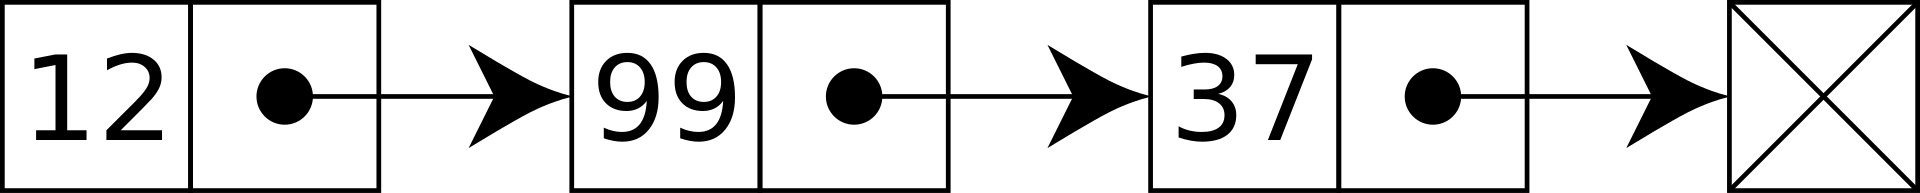
\includegraphics[scale=0.10]{Images/linked-list}
\end{center}
\end{frame}



\begin{frame}{Lesson 3}{Linked lists}
\LARGE
\textbf{Linked Lists}\\~\\
Each node contains data, and a reference (in other words, a link) to the next
node in the sequence. This structure allows for efficient insertion or removal of
elements from any position in the sequence during iteration.
\end{frame}



\begin{frame}{Lesson 3}{Linked lists}
\LARGE
\textbf{Linked Lists}\\~\\
A drawback of linked lists is that data access time is linear in respect to the
number of nodes in the list. Because nodes are serially linked, accessing any
node requires that the prior node be accessed beforehand.
\end{frame}


\begin{frame}{Lesson 3}{Linked lists}
\LARGE
\textbf{Linked Lists}\\~\\
Linked lists are among the simplest and most common data structures. They can be
used to implement several other common abstract data types, including stacks,
queues, \alert{associative and dynamic arrays}.
\end{frame}


\begin{frame}{Lesson 3}{Linked lists}
\LARGE
\textbf{Dynamic Arrays}\\~\\
Variable-size list data structure that allows elements to be added or removed. 
Dynamic arrays overcome a limit of static arrays, which have a fixed capacity
that needs to be specified at allocation. 
\end{frame}


\begin{frame}{Lesson 3}{Linked lists}
\LARGE
\textbf{Associative Arrays}\\~\\
A map, symbol table, or dictionary is an abstract data type that stores a
collection of (key, value) pairs, such that each possible key appears at most
once in the collection. It supports lookup, remove, and insert operations. 
\end{frame}


\begin{frame}{Lesson 3}{Linked lists}
\LARGE
\textbf{Associative Arrays}\\~\\
\begin{center}
\begin{hashtable}
   0 & 110 \\
   1 & 100 \\
   2 &  90 \\
   3 &  80 \\
   4 &  70 \\
   5 &  50
\end{hashtable}
\end{center}
\end{frame}


\begin{frame}{Lesson 3}{Stacks}
\Huge
Linked lists vs. Arrays
\end{frame}


\begin{frame}{Lesson 3}{}
{\LARGE\textbf{{Linked lists vs. Arrays}}}\\~\\
\noindent\begin{minipage}[t]{0.5\linewidth}
    \textbf{Linked lists}
    \begin{itemize}
    \item{Dynamic in size}
    \item{Can contain any number of nodes}
    \item{Store various data types}
    \end{itemize}
    \end{minipage}%
    \begin{minipage}[t]{0.5\linewidth}
    \textbf{Arrays}
    \begin{itemize}
    \item{Fixed in size}
    \item{Size is given at the time of creation}
    \item{Similar data types}
    \end{itemize}
\end{minipage}\par\bigskip
\end{frame}



\begin{frame}{Lesson 3}{Linked lists}
\LARGE
\textbf{Linked Lists}\\~\\
The principal benefit of a linked list over a conventional array is that the list
elements can be easily inserted or removed without reallocation or reorganization
of the entire structure because the data items do not need to be stored
contiguously in memory or on disk, while restructuring an array at run-time is a
much more expensive operation.
\end{frame}




\begin{frame}{Lesson 3}{Linked lists}
\LARGE
\textbf{Linked Lists}\\~\\
 Linked lists allow insertion and removal of nodes at any point in the list, and
 allow doing so with a constant number of operations by keeping the link previous
 to the link being added or removed in memory during list traversal. 
\end{frame}



\begin{frame}{Lesson 3}{Linked lists}
\LARGE
\textbf{Linked list Operations}\\~\\
\Large
\begin{itemize}
\item \textbf{INSERT} — Add an element to the end of the queue
\item \textbf{DELETE} — Remove an element from the front of the queue
\item \textbf{TRAVERSAL} — Check if the queue is empty
\end{itemize}
\end{frame}



\begin{frame}{Lesson 3}{Linked lists}
\begin{center}
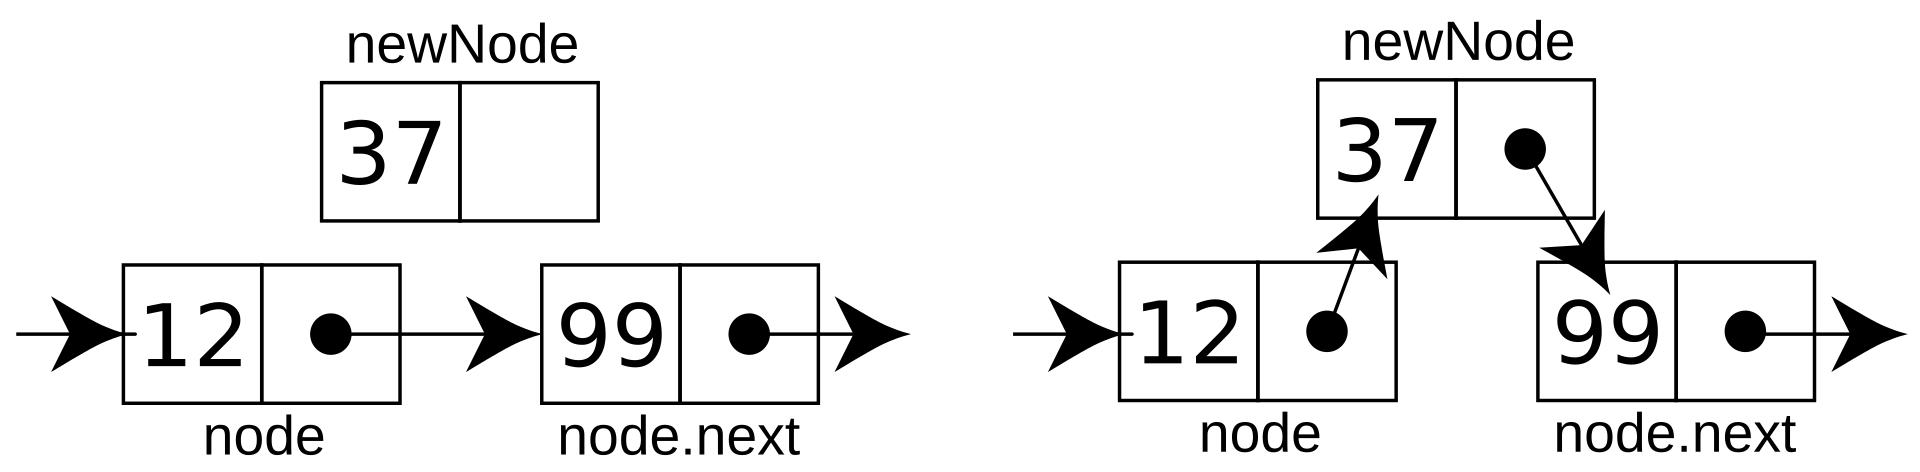
\includegraphics[scale=0.12]{Images/linkedLists-addingnode}
\end{center}
\end{frame}


\begin{frame}{Lesson 3}{Linked lists}
\begin{center}
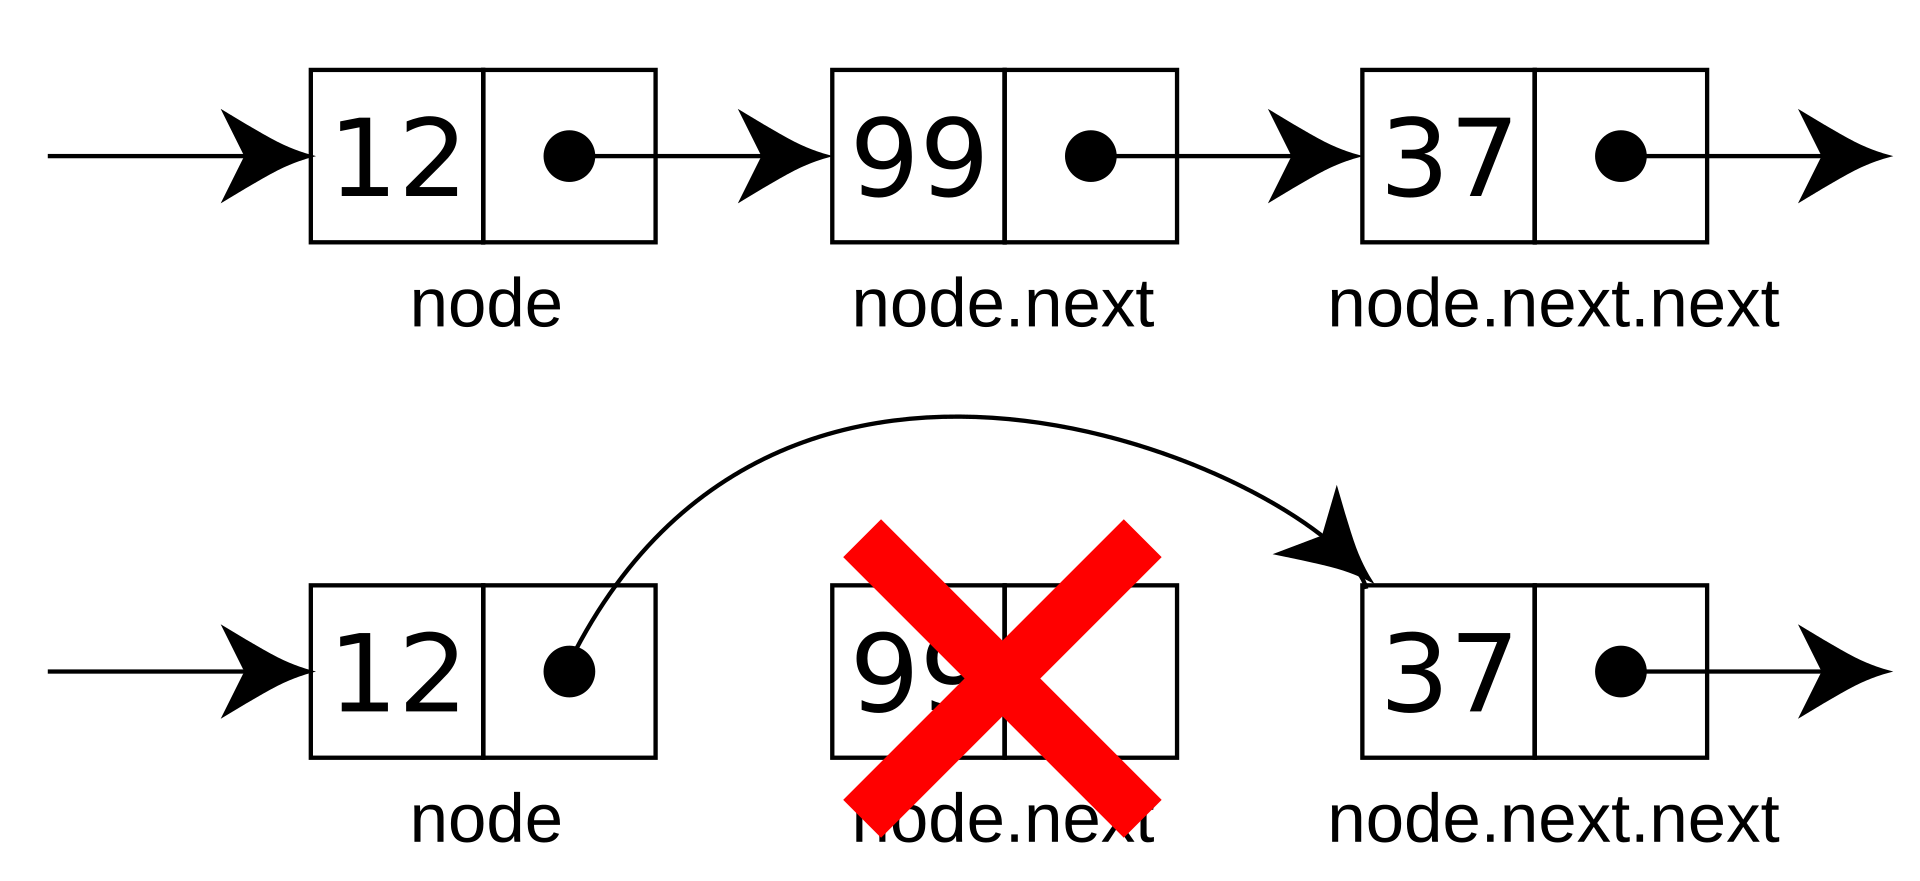
\includegraphics[scale=0.12]{Images/linkedLists-deletingnode}
\end{center}
\end{frame}


\begin{frame}{Lesson 3}{Linked lists}
\LARGE
\textbf{Linked lists}\\~\\
\Large
\begin{itemize}
	\item \textbf{Single linked list} lists contain nodes which have a value and a next pointer
\item \textbf{Double linked list} contains nodes which includes the next and previous pointer links
\item \textbf{circular linked list}  a list where the last node has a pointer to the first node
\end{itemize}
\end{frame}



\begin{frame}{Lesson 3}{Linked lists}
\LARGE
\textbf{Single Linked list}\\~\\
\begin{center}
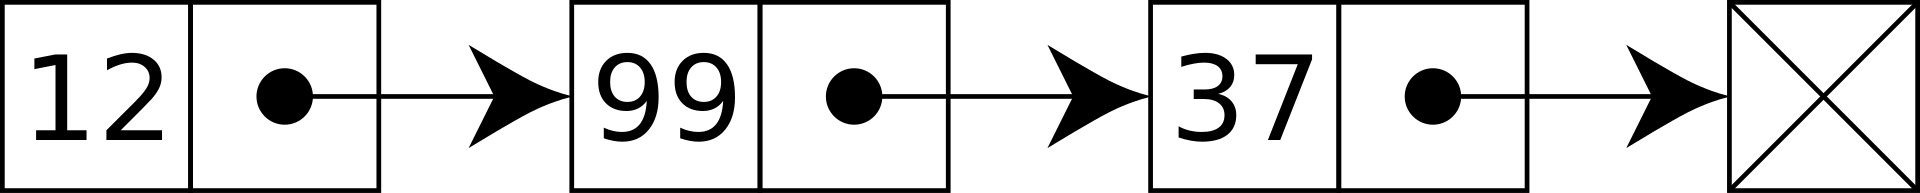
\includegraphics[scale=0.12]{Images/linked-list}
\end{center}
\end{frame}


\begin{frame}{Lesson 3}{Linked lists}
\LARGE
\textbf{Double Linked list}\\~\\
\begin{center}
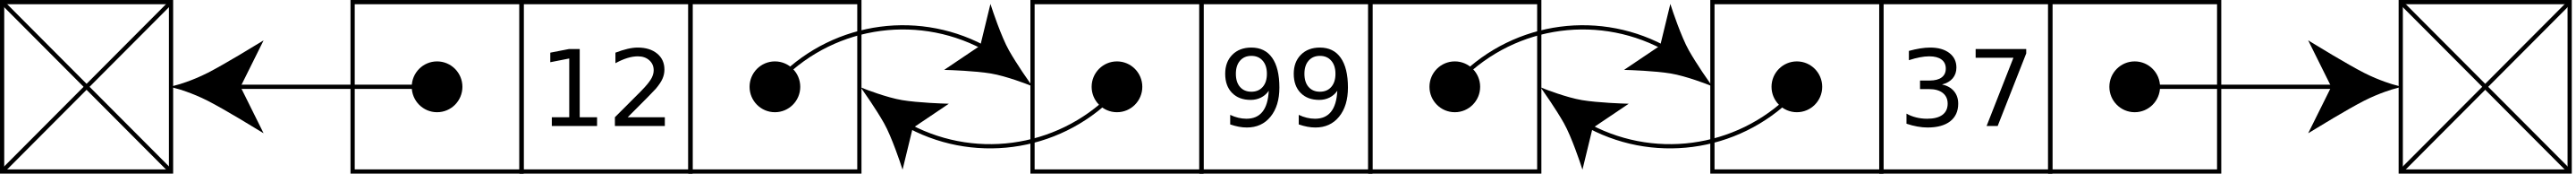
\includegraphics[scale=0.13]{Images/double-linked-list}
\end{center}
\end{frame}


\begin{frame}{Lesson 3}{Linked lists}
\LARGE
\textbf{Circular Linked list}\\~\\
\begin{center}
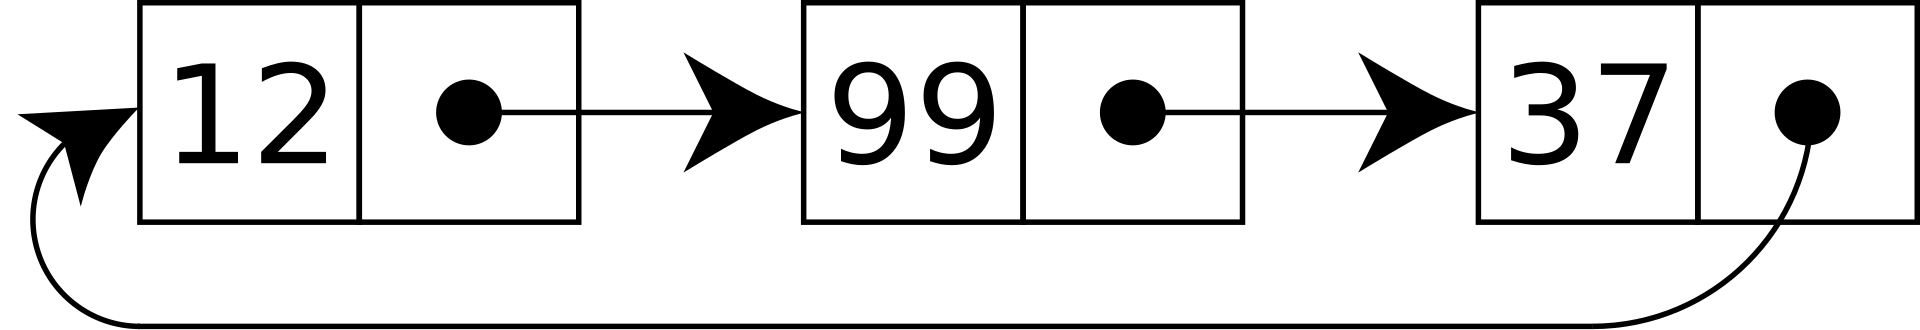
\includegraphics[scale=0.11]{Images/circular-linked-list}
\end{center}
\end{frame}



\begin{frame}[fragile]
\Large
\textbf{Linked List Example}\\
\begin{lstlisting}
# importing module 
import collections 

# initialising a deque() of arbitrary length 
linked_list = collections.deque()
# filling deque() with elements 
linked_list.append('subaru') 
linked_list.append('toyota') 
linked_list.append('mercedes') 
  
print("Elements in the linked_list:") 
print(linked_list)
\end{lstlisting}
\end{frame}





% %%%%%%%%%%%%%%%%%%%%%%%%%%%%%%%%%%%%%%%%%%%%%%%%%%%%
% Hash Table / Associative Arrays
% %%%%%%%%%%%%%%%%%%%%%%%%%%%%%%%%%%%%%%%%%%%%%%%%%%%%
\begin{frame}{Lesson 3}{Hash Table}
\begin{center}
\Huge Hash Table
\end{center}
\end{frame}


\begin{frame}{Lesson 3}{Hash Table}
\LARGE
\textbf{Linked Lists}\\~\\
A hash table is a data structure that implements an associative array, also
called a dictionary or simply map; an associative array is an abstract data type
that maps keys to values.
\end{frame}

\begin{frame}{Lesson 3}{Hash Table}
\LARGE
\textbf{Remember Associative Arrays}\\~\\
A map, symbol table, or dictionary is an abstract data type that stores a
collection of (key, value) pairs, such that each possible key appears at most
once in the collection. It supports lookup, remove, and insert operations. 
\end{frame}


\begin{frame}{Lesson 3}{Hash Table}
\LARGE
\textbf{Hash Table}\\~\\
A hash table uses a hash function to compute an index, also called a hash code,
into an array of buckets or slots, from which the desired value can be found.
During lookup, the key is hashed and the resulting hash indicates where the
corresponding value is stored. A map implemented by a hash table is called a hash
map.
\end{frame}

\begin{frame}{Lesson 3}{Hash Table}
\LARGE
\textbf{Hash Table}\\
\begin{center}
\includegraphics[scale=0.10]{Images/hash_table}
\end{center}
\end{frame}


\begin{frame}{Lesson 3}{Hash Table}
\LARGE
\textbf{Hash Table}\\~\\
Hashing concept - each key is translated by a hash function into a 
distinct index in an array. The index functions as a storage location for the
matching value. In simple words, it maps the keys with the value.
\end{frame}



\begin{frame}{Lesson 3}{Hash Table}
\LARGE
\textbf{Hash Functions: cyclic redundancy checks}\\~\\
\begin{center}
\includegraphics[scale=0.60]{Images/hash_function1}
\end{center}
\end{frame}


\begin{frame}{Lesson 3}{Hash Table}
\LARGE
\textbf{Hash Functions: checksums}\\
\begin{center}
\includegraphics[scale=0.35]{Images/hash_function2}
\end{center}
\end{frame}



\begin{frame}{Lesson 3}{Hash Table}
\LARGE
\textbf{Hash Functions: universal}\\~\\
\begin{center}
\includegraphics[scale=0.60]{Images/hash_function3}
\end{center}
\end{frame}



\begin{frame}{Lesson 3}{Hash Table}
\LARGE
\textbf{Hash Functions: keyed cryptographic}\\
\begin{center}
\includegraphics[scale=0.35]{Images/hash_function4}
\end{center}
\end{frame}


\begin{frame}{Lesson 3}{Hash Table}
\LARGE
\textbf{Hash Functions: unkeyed cryptographic}\\
\begin{center}
\includegraphics[scale=0.35]{Images/hash_function5}
\end{center}
\end{frame}



\begin{frame}{Lesson 3}{Hash Table}
\LARGE
\textbf{Hash Collisions}\\~\\
A hash collision or hash clash is when two distinct pieces of data in a hash
table share the same hash value. The hash value in this case is derived from a
hash function which takes a data input and returns a fixed length of bits.
\end{frame}


\begin{frame}{Lesson 3}{Hash Table}
\LARGE
\textbf{Hash Collisions}\\
\begin{center}
\includegraphics[scale=0.10]{Images/hash_collision}
\end{center}
\end{frame}


\begin{frame}{Lesson 3}{Hash Table}
\LARGE
\textbf{Hash Table}\\~\\
Hash tables are very much used as table lookup structures, in many kinds of
computer software, particularly database indexing, caches, and sets.
\end{frame}


\begin{frame}{Lesson 3}{Hash Table}
\LARGE
\textbf{Hash Table}\\~\\
In hash tables, since hash collisions are inevitable, hash tables have mechanisms
of dealing with them, known as collision resolutions. 
\Large
\begin{itemize}
	\item \textbf{open addressing} cells in the hash table are assigned one of three states in this method – occupied, empty, or deleted
	\item \textbf{separate chaining} allows more than one record to be chained to the cells of a hash table.
\end{itemize}
\end{frame}


\begin{frame}[fragile]
\Large
\textbf{Hash Table}\\
\begin{lstlisting}
hash_table = {"Alice": "January", "Bob": "May", "Charlie": "January"}

my_dictionary = {}
my_dictionary["Alice"] = "January" 
# Hash function determines the location for "January"

# print the key value
print(my_dictionary["Alice"]) # "January"
\end{lstlisting}
\end{frame}



% %%%%%%%%%%%%%%%%%%%%%%%%%%%%%%%%%%%%%%%%%%%%%%%%%%%%
% Trees
% %%%%%%%%%%%%%%%%%%%%%%%%%%%%%%%%%%%%%%%%%%%%%%%%%%%%
\begin{frame}{Lesson 3}{Trees}
\begin{center}
\Huge Trees
\end{center}
\end{frame}

\begin{frame}{Lesson 3}{Trees}
\LARGE
\textbf{What is a tree?}\\~\\
A tree is a very widely used abstract data type that represents a
hierarchical structure with a set of connected nodes. Each node i
the tree can be connected to many children (depending on the type of
tree), but must be connected to exactly one parent, except for the
root node, which has no parent
\end{frame}


\begin{frame}{Lesson 3}{Trees}
\LARGE
\textbf{Unsorted tree}\\
\begin{center}
\includegraphics[scale=0.12]{Images/tree1}
\end{center}
\end{frame}


\begin{frame}{Lesson 3}{Trees}
\LARGE
\textbf{Tree}\\~\\
There should be no cycles or "loops" (no node can be its own
ancestor), and also that each child can be treated like the root
node of its own subtree, making recursion a useful technique for
tree traversal.	
\end{frame}

\begin{frame}{Lesson 3}{Trees}
\LARGE
\textbf{Tree Node}\\~\\
A node is a structure which may contain data and connections to
other nodes, sometimes called edges or links. Each node in a tree
has zero or more child nodes, which are below it in the tree (by
convention, trees are drawn with descendants going downwards).
\end{frame}


\begin{frame}{Lesson 3}{Trees}
\LARGE
\textbf{Tree Node}\\~\\
A node that has a child is called the child's parent node (or
superior). All nodes have exactly one parent, except the topmost
root node, which has none. A node might have many ancestor nodes,
such as the parent's parent.
\end{frame}


\begin{frame}{Lesson 3}{Trees}
\begin{center}
\includegraphics[scale=0.15]{Images/tree3}
\end{center}
\end{frame}


\begin{frame}{Lesson 3}{Trees}
\begin{center}
\includegraphics[scale=0.60]{Images/tree4}
\end{center}
\end{frame}


\begin{frame}{Lesson 3}{Trees}
\begin{center}
\includegraphics[scale=0.10]{Images/tree5}
\end{center}
\end{frame}


\begin{frame}{Lesson 3}{Trees}
\begin{center}
\includegraphics[scale=0.10]{Images/tree2}
\end{center}
\end{frame}


\begin{frame}{Lesson 3}{Trees}
\LARGE
\textbf{Structure}\\
\begin{center}
\includegraphics[scale=0.55]{Images/tree-structure}
\end{center}
\end{frame}


\begin{frame}{Lesson 3}{Trees}
\LARGE
\textbf{Organization}
\begin{center}
\includegraphics[scale=0.48]{Images/tree-structure2}
\end{center}
\end{frame}


\begin{frame}{Lesson 3}{Trees}
\LARGE
\textbf{Tree - Properties}\\~\\
\Large
\begin{itemize}
	\item \textbf{Number of edges} as the connection between two nodes. If a tree has N nodes then it will have (N-1) edges. There is only one path from each node to any other node of the tree
	\item \textbf{Depth of a node} the length of the path from the root to that node. Each edge adds 1 unit of length to the path. So, it can also be defined as the number of edges in the path from the root of the tree to the node.
\end{itemize}
\end{frame}


\begin{frame}{Lesson 3}{Trees}
\LARGE
\textbf{Tree Properties}\\~\\
\Large
\begin{itemize}
	\item \textbf{Height of a node} as the length of the longest path from the node to a leaf node of the tree.
	\item \textbf{Height of the Tree} is the length of the longest path from the root of the tree to a leaf node of the tree
	\item \textbf{Degree of a Node} the total count of subtrees attached to that node
\end{itemize}
\end{frame}



\begin{frame}{Lesson 3}{Trees}
\LARGE
\textbf{Height vs. Depth}
\begin{center}
\includegraphics[scale=0.48]{Images/depth-height}
\end{center}
\end{frame}


\begin{frame}{Lesson 3}{Trees}
\LARGE
\textbf{Tree - Non-linear data structure}\\~\\
\begin{itemize}
	\item \textbf{not linear} data in a tree are not stored in a sequential manner
	\item \textbf{hierarchical structure} data arranged on multiple levels
\end{itemize}
\end{frame}


\begin{frame}{Lesson 3}{Trees}
\LARGE
\textbf{Types of Trees}\\~\\
\begin{itemize}
	\item \textbf{Binary tree}
	\item \textbf{Ternary Tree}
	\item \textbf{Generic Tree}
\end{itemize}
\end{frame}

\begin{frame}{Lesson 3}{Trees}
\begin{center}
\huge Binary Trees
\end{center}
\end{frame}

\begin{frame}{Lesson 3}{Trees}
\LARGE
\textbf{Binary Tree}\\~\\
A binary tree is a tree data structure in which each node has at
most two children, referred to as the left child and the right
child.
\end{frame}


\begin{frame}{Lesson 3}{Trees}
\begin{center}
\includegraphics[scale=0.60]{Images/binary-tree}
\end{center}
\end{frame}

\begin{frame}{Lesson 3}{Trees}
\LARGE
\textbf{Full Binary Tree}\\~\\
A full binary tree is a binary tree with either zero or two child
nodes for each node. 
\begin{center}
\includegraphics[scale=0.48]{Images/full-binary-tree}
\end{center}
\end{frame}


\begin{frame}{Lesson 3}{Trees}
\LARGE
\textbf{Complete Binary Tree}\\
A complete binary tree is a special type of binary tree where all
the levels of the tree are filled completely except the lowest level
nodes which are filled from as left as possible.
\begin{center}
\includegraphics[scale=0.60]{Images/complete-binary-tree}
\end{center}
\end{frame}


\begin{frame}{Lesson 3}{Trees}
\LARGE
\textbf{Perfect Binary Tree}\\
A perfect binary tree is a special type of binary tree in which all
the leaf nodes are at the same depth, and all non-leaf nodes have
two children. In simple terms, this means that all leaf nodes are at
the maximum depth of the tree, and the tree is completely filled
with no gaps.
\end{frame}


\begin{frame}{Lesson 3}{Trees}
\LARGE
\textbf{Perfect Binary Tree}\\
\begin{center}
\includegraphics[scale=0.45]{Images/perfect-binary-tree}
\end{center}
\end{frame}

\begin{frame}{Lesson 3}{Trees}
\begin{center}
\huge Ternary Trees
\end{center}
\end{frame}

\begin{frame}{Lesson 3}{Trees}
\LARGE
\textbf{Ternary Tree}\\~\\
\begin{center}
\includegraphics[scale=0.48]{Images/ternary-tree}
\end{center}
\end{frame}

\begin{frame}{Lesson 3}{Trees}
\begin{center}
\huge Generic Trees
\end{center}
\end{frame}

\begin{frame}{Lesson 3}{Trees}
\LARGE
\textbf{Generic Tree}\\~\\
\begin{center}
\includegraphics[scale=0.55]{Images/generic-tree}
\end{center}
\end{frame}

\begin{frame}{Lesson 3}{Trees}
\begin{center}
\includegraphics[scale=0.55]{Images/tree-types}
\end{center}
\end{frame}


\begin{frame}{Lesson 3}{Trees}
\LARGE
\textbf{Binary search tree (BST)}\\
A B-Tree is a specialized N-way tree designed to optimize data
access, especially on disk-based storage systems.
\begin{center}
\includegraphics[scale=0.65]{Images/btree}
\end{center}
\end{frame}

\begin{frame}{Lesson 3}{Trees}
\LARGE
\textbf{Binary Search Trees (BST)}\\~\\
\Large
A B-tree is a \alert{self-balancing} tree data structure that
maintains sorted data and allows searches, sequential access,
insertions, and deletions very fast (logarithmic time). The B-tree
generalizes the binary search tree, allowing for nodes with more
than two children.
\end{frame}


\begin{frame}{Lesson 3}{Trees}
\LARGE
\textbf{Self-Balancing?}\\~\\
\Large
A self-balancing tree is a tree that automatically keeps its height
(maximal number of levels below the root) small in the face of
arbitrary item insertions and deletions.
\end{frame}


\begin{frame}{Lesson 3}{Trees}
\LARGE
\textbf{Un-balanced tree}\\~\\
\begin{center}
\includegraphics[scale=0.10]{Images/unbalanced-tree}
\end{center}
\end{frame}



\begin{frame}{Lesson 3}{Trees}
\LARGE
\textbf{Self-balanced tree}\\~\\
\begin{center}
\includegraphics[scale=0.10]{Images/selfbalanced-tree}
\end{center}
\end{frame}


\begin{frame}{Lesson 3}{Trees}
\LARGE
\textbf{Binary Search Trees (BST)}\\~\\
\Large
Binary search trees allow very fast lookup, addition, and removal of
data items using binary search. Binary search trees are the basis
and very important for sorting and search algorithms.
\end{frame}


\begin{frame}{Lesson 3}{Trees}
\LARGE
\textbf{Tree Operations}\\~\\
\Large
\begin{itemize}
\item \textbf{CREATE} — create a tree in a data structure
\item \textbf{INSERT} — insert data in a tree
\item \textbf{SEARCH} — search data in a tree
\item \textbf{TRAVERSAL} — Depth-First, Breadth-First
\end{itemize}
\end{frame}


\begin{frame}{Lesson 3}{Trees}
\LARGE
\textbf{There are numerous applications of trees}\\
\Large
\begin{itemize}
    \item File system implementation: directory structure
    \item Natural language processing (NLP)
    \item AI, Genetic programming
    \item Database indexing (BST B-Trees, B+ Trees)
\end{itemize}
\end{frame}



% %%%%%%%%%%%%%%%%%%%%%%%%%%%%%%%%%%%%%%%%%%%%%%%%%%%%
% Graphs
% %%%%%%%%%%%%%%%%%%%%%%%%%%%%%%%%%%%%%%%%%%%%%%%%%%%%
\begin{frame}{Lesson 3}{Graphs}
\begin{center}
\Huge Graphs
\end{center}
\end{frame}

\begin{frame}{Lesson 3}{Graphs}
\LARGE
\textbf{What is a graph?}\\~\\
A graph is a non-linear data structure consisting of vertices and
edges. It is an abstract data type that consists of a finite set of
vertices (nodes or points), together with a set of edges (also
called links or lines).
\end{frame}


\begin{frame}{Lesson 3}{Graphs}
\LARGE
\textbf{Graphs}\\
\begin{center}
\includegraphics[scale=0.10]{Images/graph}
\end{center}
\end{frame}


\begin{frame}{Lesson 3}{Graphs}
\LARGE
\textbf{Graphs vs Trees}\\
\begin{center}
\includegraphics[scale=0.45]{Images/treevsgraph}
\end{center}
\end{frame}


\begin{frame}{Lesson 3}{Graphs}
\LARGE
\textbf{Graphs}\\~\\
A graph data structure is a collection of nodes (also called
vertices) and edges that connect them. Nodes can represent entities,
such as people, places, or things, while edges represent
relationships between those entities.
\end{frame}



\begin{frame}{Lesson 3}{Graphs}
\LARGE
\textbf{Trees}\\~\\
A tree data structure is a hierarchical data structure that consists
of nodes connected by edges. Each node can have multiple child
nodes, but only one parent node. The topmost node in the tree is
called the root node.
\end{frame}


\begin{frame}{Lesson 3}{Graphs}
\begin{center}
\includegraphics[scale=0.35]{Images/treevsgraph2}
\end{center}
\end{frame}


\begin{frame}{Lesson 3}{Graphs}
\LARGE
\textbf{Graphs vs Trees}\\
\Large
\begin{itemize}
    \item \textbf{Cycles} Graphs can contain cycles, while trees cannot
    \item \textbf{Connectivity} Graphs can be disconnected, while trees are always connected
    \item \textbf{Hierarchy} Trees have a hierarchical structure, with one vertex designated as the root. Graphs do not have this hierarchical structure
    \item \textbf{Applications} Trees used in hierarchical data structures, such as file systems and XML documents. Graphs better for modelling transportation networks, social networks, computer networks
\end{itemize}
\end{frame}



\begin{frame}{Lesson 3}{Graphs}
\LARGE
\textbf{Types of graphs}\\~\\
\Large
\begin{itemize}
	\item \textbf{Directed and Undirected graphs}
	\item \textbf{Weighted Vs Unweighted graphs}
\end{itemize}
\end{frame}



\begin{frame}{Lesson 3}{Graphs}
\LARGE
\textbf{Directed graph}\\
A directed graph is defined as a type of graph where the edges have
a direction associated with them.
\begin{center}
\includegraphics[scale=0.65]{Images/directed-graph}
\end{center}
\end{frame}



\begin{frame}{Lesson 3}{Graphs}
\LARGE
\textbf{Directed graphs}\\~\\
\Large
\begin{itemize}
	\item edges have a direction associated with them, indicating a one-way relationship between vertices
	\item each vertex in a directed graph has two different degree measures: indegree and outdegree. Indegree is the number of incoming edges to a vertex, while outdegree is the number of outgoing edges from a vertex
	\item A directed graph can contain cycles, which are paths that start and end at the same vertex and contain at least one edge
\end{itemize}
\end{frame}


\begin{frame}{Lesson 3}{Graphs}
\LARGE
\textbf{There are numerous applications of directed graphs}\\
\Large
\begin{itemize}
    \item social networks
    \item transportation networks: flight routes, railroads, and road networks. Cities, towns, and intersections are represented by nodes, and the links that connect these locations—such as highways, train tracks, and flight routes—are represented by edges.
    \item computer networks
\end{itemize}
\end{frame}


\begin{frame}{Lesson 3}{Graphs}
\LARGE
\textbf{Undirected graph}\\
An undirected graph is a type of graph where the edges have no
specified direction assigned to the them.
\begin{center}
\includegraphics[scale=0.65]{Images/undirected-graph}
\end{center}
\end{frame}


\begin{frame}{Lesson 3}{Graphs}
\LARGE
\textbf{Undirected graphs}\\~\\
\Large
\begin{itemize}
	\item edges in an undirected graph are bidirectional
	\item there is no concept of a “parent” or “child” vertex as there is no direction to the edges.
	\item may contain loops, which are edges that connect a vertex to itself
\end{itemize}
\end{frame}


\begin{frame}{Lesson 3}{Graphs}
\LARGE
\textbf{Applications of un-directed graphs}\\
\Large
\begin{itemize}
    \item traffic flow optimization: Undirected graphs are used in traffic flow optimization to model the flow of vehicles on road networks. The vertices of the graph represent intersections or road segments, and the edges represent the connections between them. The graph can be used to optimize traffic flow and plan transportation infrastructure
    \item website analysis: analyze the links between web pages on the internet
\end{itemize}
\end{frame}



\begin{frame}{Lesson 3}{Graphs}
\LARGE
\textbf{Weighted graph}\\
A weighted graph is defined as a special type of graph in which the
edges are assigned some weights which represent cost, distance, and
many other relative measuring units.
\begin{center}
\includegraphics[scale=0.45]{Images/weighted-graph}
\end{center}
\end{frame}


\begin{frame}{Lesson 3}{Graphs}
\LARGE
\textbf{Applications of weighted graphs}\\
\Large
\begin{itemize}
    \item Transportation networks: solve the path that takes the least time, or the path with the least overall distance. This is a simplification of how weighted graphs can be used for more complex things like a GPS system. Graphs are used to study traffic patterns, traffic light timings and much more by many big tech companies such as UBER etc. Graph networks are used by many map programs such as Google Maps, Bing Maps
    \item Epidemiology: Weighted graphs can be used to find the maximum distance transmission from an infectious to a healthy person
\end{itemize}
\end{frame}




\begin{frame}{Lesson 3}{Graphs}
\LARGE
\textbf{Unweighted graph}\\
An unweighted graph is a graph in which the edges do not have
weights or costs associated with them. Instead, they simply
represent the presence of a connection between two vertices.
\begin{center}
\includegraphics[scale=0.65]{Images/unweighted-graph}
\end{center}
\end{frame}



\begin{frame}{Lesson 3}{Graphs}
\LARGE
\textbf{Applications of unweighted graphs}\\
\Large
\begin{itemize}
    \item represent circuit diagrams
    \item solve puzzles    
    \item used in social media sites to find whether two users are connected or not
    \item can modelate the possible moves in a game
\end{itemize}
\end{frame}


\begin{frame}{Lesson 3}{Graphs}
\LARGE
\textbf{A real problem}\\
Given a list of cities and the distances between each pair of
cities, what is the shortest possible route that visits each city
exactly once and returns to the origin city?
\begin{center}
\includegraphics[scale=0.55]{Images/tsp}
\end{center}
\end{frame}


\begin{frame}{Lesson 3}{Graphs}
\LARGE
\textbf{How we plan to solve the problem?}\\~\\
\begin{itemize}
    \item think how we represent the problem
    \item what data structure we plan to use
    \item and what algorithm
\end{itemize}
\end{frame}



\begin{frame}{Lesson 3}{Graphs}
\LARGE
\textbf{TSP Example 1}\\
\begin{center}
\includegraphics[scale=0.35]{Images/tsp0}
\end{center}
\end{frame}


\begin{frame}{Lesson 3}{Graphs}
\LARGE
\textbf{TSP Example 2}\\
\begin{center}
\includegraphics[scale=0.40]{Images/tsp1}
\end{center}
\end{frame}


\begin{frame}{Lesson 3}{Graphs}
\LARGE
\textbf{TSP Example 3}
\begin{center}
\includegraphics[scale=0.33]{Images/tsp2}
\end{center}
\end{frame}


\begin{frame}{Lesson 3}{Graphs}
\LARGE
\textbf{TSP Original Problem}\\
\begin{center}
\includegraphics[scale=0.65]{Images/tsp}
\end{center}
\end{frame}


\begin{frame}{Lesson 3}{Graphs}
\LARGE
\textbf{Why TSP matters?}\\
\Large
It represents real-world problems:
\begin{itemize}
    \item Delivery services need to plan routes to drop off packages at multiple locations
    \item Logistics companies need to find the shortest path to transport goods efficiently
    \item Manufacturing companies need to reduce the travel of robotic arms in factories
    \item Solving TSP helps reduce time, fuel costs, and energy, making operations faster and cheaper
\end{itemize}
\end{frame}


\begin{frame}{Lesson 3}{Graphs}
\Huge
How to solve it?
\end{frame}


\begin{frame}{Lesson 3}{Graphs}
\LARGE
\textbf{How to solve TSP?}\\~\\
\Large
\begin{itemize}
	\item Brute-Force Approach
	\item Dynamic Programming
	\item Approximation Algorithms
\end{itemize}
\end{frame}



\begin{frame}{Lesson 3}{Graphs}
\LARGE
\textbf{Brute-Force Approach}\\~\\
\Large
This method explores all possible routes (permutations) between
cities, calculates the total distance for each route, and selects
the shortest one. It guarantees an optimal solution but is
inefficient.
\begin{itemize}
	\item Advantages: Guarantees the optimal solution
	\item Disadvantages: Extremely slow for large datasets due to factorial growth in possible routes
\end{itemize}
\end{frame}


\begin{frame}{Lesson 3}{Graphs}
\LARGE
\textbf{Dynamic Programming}\\~\\
\Large
The travelling salesman problem using dynamic programming breaks the
problem into smaller subproblems. It solves these subproblems and
stores the results to avoid redundant calculations.
\begin{itemize}
	\item Advantages: More efficient than brute-force and provides an exact solution
	\item Disadvantages:  Still exponential, making it impractical for large numbers of cities, though it performs better than brute-force
\end{itemize}
\end{frame}


\begin{frame}{Lesson 3}{Graphs}
\LARGE
\textbf{How to solve TSP?}\\
\begin{center}
\includegraphics[scale=0.60]{Images/solve-tsp}
\end{center}
\end{frame}


\begin{frame}{Lesson 3}{Graphs}
\LARGE
\textbf{Travelling salesman problem (TSP)}\\~\\
\Large
It is an \alert{NP-hard} problem in combinatorial optimization,
important in theoretical computer science and operations research.
Applications: the travelling purchaser problem, the vehicle routing
problem and the ring star problem are three generalizations of TSP.
\end{frame}



\begin{frame}{Lesson 3}{Graphs}
\Huge
\begin{center}
NP-Hard problem?
\end{center}
\end{frame}


% %%%%%%%%%%%%%%%%%%%%%%%%%%%%%%%%%%%%%%%%%%% %
% Algorithm Complexity                        %
% %%%%%%%%%%%%%%%%%%%%%%%%%%%%%%%%%%%%%%%%%%% %

\begin{frame}{Lesson 3}{}
\begin{center}
\Huge \textbf{Algorithm Complexity}
\end{center}
\end{frame}


\begin{frame}{Lesson 3}{Graphs}
\Huge
\begin{center}
What is a NP-Hard problem?
\end{center}
\end{frame}


\begin{frame}{Lesson 3}{Algorithm Complexity}
\LARGE
\textbf{Computational problems}\\~\\
There are problems which can be solved simple way and problems which 
might not be simple to solve at all, but still for which we can find an 
algorithm to solve them.\\~\\
\textbf{And there are problems for which we cant find an algorithm at all to
solve them.}
\end{frame}



\begin{frame}{Lesson 3}{Algorithm Complexity}
\LARGE
\textbf{Problem classification}\\~\\
Computational complexity theory focuses on classifying computational problems, 
describing all possible algorithms that could be used to solve them. It tries to
classify problems that can or cannot be solved.
\end{frame}
 
 

\begin{frame}{Lesson 3}{Algorithm Complexity}
\LARGE
\textbf{Complexity Classes}\\~\\
In CS, problems are divided into classes known as Complexity
classes. A Complexity Class is a set of problems, which can be solved 
by computers depending on their related complexity.
\Large
\begin{itemize}
	\item Problems that can be efficiently solved (Polynomial time)
	\item Problems with no efficient solution (Exponential time)
	\item Problems that cannot be solved by computers
\end{itemize}
\end{frame}


\begin{frame}{Lesson 3}{Algorithm Complexity}
\LARGE
\textbf{Complexity Classes. Types}\\
\begin{center}
\includegraphics[scale=0.35]{Images/np-hard}
\end{center}
\end{frame}


\begin{frame}{Lesson 3}{Algorithm Complexity}
\LARGE
\textbf{Complexity Classes. Types}\\~\\
\Large
\begin{itemize}
	\item \textbf{P class}: Polynomial Time. Problems that can be solved by an algorithm in polynomial time. In other words, the time taken to solve these problems grows at a polynomial rate as the input size increases.
	\item \textbf{NP class}: Non-deterministic Polynomial Time. Problems in class NP are those where a solution can be verified in polynomial time, but we don’t necessarily know how to solve them efficiently.	
    \item \textbf{NP-Hard}: NP-Hard problems are at least as hard as the hardest problems in NP, but they may not even belong to class NP.
\end{itemize}
\end{frame}


\begin{frame}{Lesson 3}{Algorithm Complexity}
\LARGE
\textbf{Complexity Classes. P class}\\~\\
\Large
Problems in class P are those that can be solved by an algorithm in polynomial
time. In other words, the time taken to solve these problems grows at a polynomial
rate as the input size increases. Polynomial time algorithms are considered
efficient and practical for real-world use. 
\textbf{If a problem is in class P, it means we can solve it relatively quickly
even for large inputs.}
\end{frame}


\begin{frame}{Lesson 3}{Algorithm Complexity}
\LARGE
\textbf{Complexity Classes. NP class}\\~\\
\Large
Problems in class NP are those where a solution can be verified in polynomial
time, but we don’t necessarily know how to solve them efficiently. The key idea
here is that if someone gives us a solution, we can check if it’s correct in a
reasonable amount of time.
\textbf{NP problems are crucial because they are often more challenging to solve
but still easy to verify. Easy means Polynomial time.}
\end{frame}



\begin{frame}{Lesson 3}{Algorithm Complexity}
\LARGE
\textbf{A problem is in NP if it is easy to verify its solutions.}
\end{frame}




\begin{frame}{Lesson 3}{Algorithm Complexity}
\LARGE
\textbf{Complexity Classes. NP-Hard class}\\~\\
\Large
NP-Hard problems are at least as hard as the hardest problems in NP, but they may
not even belong to class NP. 
\textbf{We could develop an algorithm to solve the problem, but once it’s
executed, it keeps running endlessly without ever stopping. That would only 
happen if you use a large input for a given problem.}
\end{frame}


\begin{frame}{Lesson 3}{Algorithm Complexity}
\LARGE
\textbf{A problem is NP-hard if it is difficult to solve, or find a solution.}
\end{frame}





\begin{frame}{Lesson 3}{Algorithm Complexity}
\LARGE
\textbf{Complexity Classes. NP-Hard class}\\~\\
\Large
Example: trying to solve a traveling salesman problem and you input 1000 cities,
expecting to get a solution, it won’t happen. You’ve essentially set the program
to run indefinitely, and it will take about 240 years to solve if you have a super
computer.
\end{frame}



\begin{frame}{Lesson 3}{Algorithm Complexity}
\LARGE
\textbf{Complexity Classes}\\~\\
\Large
An algorithm having time complexity of the form $O(n^k)$ for input n
and constant k is called polynomial time solution. These solutions scale well.
\\~\\
On the other hand, time complexity of the form $O(k^n)$ is exponential time.
\end{frame}



\begin{frame}{Lesson 3}{Algorithm Complexity}
\LARGE
\textbf{Polynomial Time}\\~\\
\Large
An algorithm is said to be of polynomial time if its running time is upper bounded
by a \alert{polynomial} expression in the size of the input for the algorithm,
that is $T(n) = O(n^k)$ for some positive constant k.
\end{frame}


\begin{frame}{Lesson 3}{Algorithm Complexity}
\LARGE
\textbf{What is Polynomial Complexity?}\\~\\
An algorithm is said to have polynomial complexity if its resource usage can be
expressed as a polynomial function of the input size, n. Formally, an algorithm
has polynomial time complexity if its running time is $O(n^k)$ for some non
negative integer k.
\end{frame}


\begin{frame}{Lesson 3}{Algorithm Complexity}
\LARGE
\textbf{Polynomial expression}\\~\\
\Large
In mathematics, a polynomial is a mathematical expression consisting of variables
and coefficients, that involves only the operations of addition, subtraction,
multiplication and exponentiation to nonnegative integer powers, and has a finite
number of terms. An example of a polynomial of a single indeterminate x is 
\(x^2 + 3x - 5\)
\end{frame}


\begin{frame}{Lesson 3}{Algorithm Complexity}
\LARGE
\textbf{Polynomial of degree 0 \(f(x)=2\)}\\
\begin{center}
\includegraphics[scale=0.10]{Images/polynom-deg0}
\end{center}
\end{frame}



\begin{frame}{Lesson 3}{Algorithm Complexity}
\LARGE
\textbf{Polynomial of degree 1 \(f(x) = 2x + 1\)}\\
\begin{center}
\includegraphics[scale=0.55]{Images/polynom-deg1}
\end{center}
\end{frame}


\begin{frame}{Lesson 3}{Algorithm Complexity}
\LARGE
\textbf{Polynomial of degree 2 }\\
\begin{center}
\includegraphics[scale=0.10]{Images/polynom-deg2}
\end{center}
\end{frame}



\begin{frame}{Lesson 3}{Algorithm Complexity}
\LARGE
\textbf{Characteristics of Polynomial Complexity}\\
\Large
\begin{itemize}
	\item Predictable Growth: The growth rate of polynomial functions is predictable and manageable for small to moderate input sizes.
	\item Efficient for Larger Inputs: Algorithms with polynomial complexity are generally considered efficient and scalable.
	\item Classification: Polynomial time algorithms are categorized based on their degree: Linear Time $O(n)$: The simplest form, where the running time increases directly with the input size.
	\item Quadratic Time $O(n^2)$: The running time increases with the square of the input size.
\end{itemize}
\end{frame}




\begin{frame}{Lesson 3}{Algorithm Complexity}
\LARGE
\textbf{Polynomial Time}\\
\Large
Some examples of polynomial-time algorithms:
\begin{itemize}
	\item Linear search, selection sort sorting algorithm 
	\item Bubble sort
	\item All the basic arithmetic operations (addition, subtraction, multiplication, division, and comparison) can be done in polynomial time.
	\item Maximum matchings in graphs can be found in polynomial time. In some contexts, especially in optimization, one differentiates between strongly polynomial time and weakly polynomial time algorithms.
\end{itemize}
\end{frame}



\begin{frame}{Lesson 3}{Algorithm Complexity}
\LARGE
\textbf{Exponential Time}\\~\\
\Large
An algorithm is said to be exponential time, if T(n) is upper bounded by
\(2^{poly(n)}\), where poly is some polynomial in n.
\end{frame}



\begin{frame}{Lesson 3}{Algorithm Complexity}
\LARGE
\textbf{What is Exponential Complexity?}\\~\\
An algorithm has exponential complexity if its resource usage can be expressed as
an exponential function of the input size, typically $O(2^n)$ or $O(c^n)$ for some
constant $c>1$.
\end{frame}





\begin{frame}{Lesson 3}{Algorithm Complexity}
\LARGE
\textbf{Characteristics of Exponential Complexity}\\~\\
\Large
\begin{itemize}
	\item Rapid Growth: Exponential functions grow much faster than polynomial functions. Even for relatively small input sizes, the resource requirements can become impractically large.
	\item Hard to control: Algorithms with exponential complexity are generally considered hard to control for large input sizes.	
    \item Resource Exhaustion: Due to the rapid growth in resource requirements, these algorithms often become infeasible as the input size increase.
\end{itemize}
\end{frame}



\begin{frame}{Lesson 3}{Algorithm Complexity}
\LARGE
\textbf{Algorithm Complexity}\\~\\
A computational problem is a task solved by a computer. A
computation problem is solvable by an algorithm.\\~\\
\Large
\textbf{Computational complexity theory focuses on classifying
computational problems according to their resource usage, and
explores the relationships between these classifications}
\end{frame}
 

\begin{frame}{Lesson 3}{Algorithm Complexity}
\LARGE
\textbf{Algorithm Complexity}\\~\\
\Large
A problem is regarded as difficult if its solution requires significant 
resources, whatever the algorithm used. The theory formalizes this intuition, 
by introducing mathematical models of computation to study these problems and
quantifying their computational complexity, i.e., the amount of resources 
needed to solve them, such as time and storage.
\end{frame}



\begin{frame}{Lesson 3}{Algorithm Complexity}
\LARGE
\textbf{What is Algorithm Complexity Analysis?}\\~\\
\Large
The primary motive to use data structures and algorithms (DSA) is to 
\alert{solve} a problem effectively and efficiently. But how can you decide 
if a program is efficient or not? We measure that by analysing the algorithm
complexity.
\end{frame}



\begin{frame}{Lesson 3}{Algorithm Complexity}
\LARGE
\textbf{Algorithm Complexity}\\~\\
\Large
The \alert{time complexity} of an algorithm is used to describe the 
number of steps required to solve a problem, but it can also be used
to describe how long it takes to verify the answer (the running time
of your algorithm)\\~\\
The \alert{space complexity} of an algorithm describes how much memory is
required for the algorithm to operate. 
\end{frame}



\begin{frame}{Lesson 3}{Algorithm Complexity}
\LARGE
\textbf{Space complexity}\\~\\
The space complexity of an algorithm is the space taken by an algorithm 
to run the program for a given input size. The program has some space 
requirements necessary for its execution these include auxiliary space 
and input space.\\~\\
\Large
\textbf{the space taken by the algorithm to run for a given input size}
\end{frame}




\begin{frame}{Lesson 3}{Algorithm Complexity}
\LARGE
\textbf{Time complexity}\\~\\
Time complexity is the computational complexity that describes the
amount of computer time it takes to run an algorithm. Time
complexity is commonly estimated by counting the number of
elementary operations performed by the algorithm, supposing that
each elementary operation takes a fixed amount of time to perform.
\end{frame}

\begin{frame}{Lesson 3}{Algorithm Complexity}
\LARGE
\textbf{Time complexity}\\~\\
Time algorithmic complexity is a measure of how long an algorithm would take to 
complete given an input of size n. If an algorithm has to scale, it should 
compute the result within a finite and practical time bound even for 
large values of n.
\end{frame}


\begin{frame}{Lesson 3}{Algorithm Complexity}
\LARGE
\textbf{Time complexity}\\~\\
To be able to select the best algorithm, calculation of complexity and time 
consumption of an algorithm is important. Thats why we need to take into
consideration time complexity analysis.
\end{frame}



\begin{frame}{Lesson 3}{Algorithm Complexity}
\LARGE
\textbf{Time complexity}\\~\\
There are 3 type of time complexity analysis (notations):
\Large
\begin{itemize}
	\item \textbf{Big-O}: Denotes the upper bound of any algorithm’s runtime, the time is taken by the algorithm in the worst case.
	\item \textbf{Big-Omega}: Denotes the best runtime of an algorithm
	\item \textbf{Big-Theta}: Denotes average case time complexity
\end{itemize}

\end{frame}


 
\begin{frame}{Lesson 3}{Algorithm Complexity}
\LARGE
\textbf{Analysis of algorithms}\\~\\
\Large
Analyzing the amount of resources needed by a particular algorithm to solve a 
problem.
\end{frame}


\begin{frame}{Lesson 3}{Algorithm Complexity}
\LARGE
\textbf{Complexity Classes}\\~\\
\Large
The common resources required by a solution are \textbf{time} and
\textbf{space}, meaning how much time the algorithm takes to solve 
a problem and the corresponding memory usage.
\end{frame}




\begin{frame}{Lesson 3}{}
\begin{center}
\huge \textbf{Big-O notation}
\end{center}
\end{frame}


\begin{frame}{Lesson 3}{Algorithm Complexity}
\LARGE
\textbf{Big-O Notation}\\~\\
\Large
Big-O notation is the most common notation to represent algorithmic complexity. 
It gives an upper bound on complexity and hence it signifies the worst-case
performance of the algorithm. With such a notation, it's easy to compare different
algorithms because the notation tells clearly how the algorithm scales when 
input size increases. This is often called the order of growth.
\end{frame}


\begin{frame}{Lesson 3}{Algorithm Complexity}
\begin{center}
\huge Big-O notation helps us answer the question, “Will it scale?”\\~\\
\Large 
Describes the upper bound of any algorithm’s runtime, example the time is taken by
the algorithm in the worst case.
\end{center}
\end{frame}


\begin{frame}{Lesson 3}{Algorithm Complexity}
\LARGE
\textbf{Constant time $O(1)$ - Excellent/Best}\\~\\
The algorithm runs for the same amount of time every time irrespective of the
input size. We call this, constant time complexity.\\~\\
\Large
For example, accessing an element in an array by index, searching for the first
word in a dictionary. Same way, joining the end of a queue in a bank is of
constant complexity regardless of how long the queue is.
\end{frame}


\begin{frame}{Lesson 3}{Algorithm Complexity}
\LARGE
\textbf{Constant time $O(1)$}\\~\\
\begin{center}
\includegraphics[scale=0.10]{Images/polynom-deg0}
\end{center}
\end{frame}


\begin{frame}{Lesson 3}{Algorithm Complexity}
\LARGE
\textbf{Logarithmic time $O(log n)$ - Good}\\~\\
When the algorithm runtime increases very slowly compared to an increase 
in input size, we say the algorithm is of logarithmic time complexity.
\end{frame}


\begin{frame}{Lesson 3}{Algorithm Complexity}
\LARGE
\textbf{Logarithmic time $O(log n)$ - Good}\\~\\
\begin{center}
\includegraphics[scale=0.30]{Images/log-function}
\end{center}
\end{frame}


\begin{frame}{Lesson 3}{Algorithm Complexity}
\LARGE
\textbf{Linear time - $O(n)$- Fair}\\~\\
If the algorithm runtime is linearly proportional to the input size then we call 
the algorithm to be of linear time complexity.
\\~\\
\Large
We are looking for a specific item in a long unsorted list. We will probable
compare each item. Search time is proportional to the list size. Here we say the
complexity is to be \textbf{linear}.
\end{frame}


\begin{frame}{Lesson 3}{Algorithm Complexity}
\LARGE
\textbf{Linear time - $O(n)$- Fair}\\~\\
\begin{center}
\includegraphics[scale=0.08]{Images/linear-function}
\end{center}
\end{frame}


\begin{frame}{Lesson 3}{Algorithm Complexity}
\LARGE
\textbf{Log-Liner time $O(n log n)$ - Bad}\\~\\
\end{frame}


\begin{frame}{Lesson 3}{Algorithm Complexity}
\LARGE
\textbf{Quadratic time $O(n^2)$ - Very bad}\\~\\
If we are planning to find all duplicates in an unsorted list then the complexity
becomes quadratic. Checking for duplicates for one item is of linear complexity.
But if we do this for all items, complexity becomes quadratic. Similarly, if all
people in a room are asked to shake hands with every other person, the complexity 
\textbf{quadratic}.
\end{frame}


\begin{frame}{Lesson 3}{Algorithm Complexity}
\LARGE
\textbf{Exponential time $O(2^n)$ - Horrible}\\~\\
\end{frame}


\begin{frame}{Lesson 3}{Algorithm Complexity}
\LARGE
\textbf{Factorial time $O(n!)$ - Worst}\\~\\
\end{frame}



\begin{frame}{Lesson 3}{Algorithm Complexity}
\LARGE
\textbf{Time complexity}\\
\begin{center}
\includegraphics[scale=0.25]{Images/time-complexity}
\end{center}
\end{frame}


\begin{frame}{Lesson 3}{Algorithm Complexity}
\LARGE
\textbf{Travelling salesman problem (TSP). NP-Hard}\\~\\
TSP is considered an NP-hard problem, meaning that the time required to find the
optimal solution increases exponentially as the number of cities grows.
\end{frame}




\begin{frame}{Lesson 3}{Algorithm Complexity}
\LARGE
\textbf{Travelling salesman problem (TSP). Brute-force}\\~\\
If we start to solve this problem using the brute-force method is SLOW. 
Very slow.\\
\Large
Brute force? Involves evaluating every possible permutation of cities to identify
the shortest route. This method has a factorial runtime $O(n!)$, making it 
impractical even for moderately sized datasets. For example, with just 20 cities,
there are over 2.4 quintillion ($10^18$) possible routes!
\end{frame}


\begin{frame}{Lesson 3}{Algorithm Complexity}
\LARGE
\textbf{Travelling salesman problem (TSP). Brute-force}\\~\\
Suitable only for a small network with few cities
\end{frame}


\begin{frame}{Lesson 3}{Algorithm Complexity}
\LARGE
\textbf{Travelling salesman problem (TSP). Dynamic Programming}\\~\\
The Held-Karp Algorithm\\
\Large
It offers a more efficient solution using dynamic programming. It reduces 
the time complexity to $O(n^2 * 2^n)$, which is significantly better than 
brute force but still exponential. While feasible for smaller datasets, 
the Held-Karp algorithm becomes impractical as the number of cities grows.
\end{frame}


\begin{frame}{Lesson 3}{Algorithm Complexity}
\LARGE
\textbf{Travelling salesman problem (TSP). Dynamic programming}\\~\\
Suitable for an average network with aprox 50 cities
\end{frame}


\begin{frame}{Lesson 3}{Algorithm Complexity}
\LARGE
\textbf{Travelling salesman problem (TSP). Polynomial Time}\\~\\
The holy grail of TSP research is a polynomial-time algorithm—one that can solve
the problem efficiently as the number of cities increases. Despite extensive
efforts, no such algorithm exists for the general case of the TSP. This remains 
research and development, in the context of the P vs NP problem.
\end{frame}



\begin{frame}{Lesson 3}{Algorithm Complexity}
\huge
Why should we care about an algorithm's performance when we have cloud and
processors are getting faster and memories are getting cheaper and cheaper?
\end{frame}


\begin{frame}{Lesson 3}{Algorithm Complexity}
\LARGE
\textbf{Solving the problem!}\\~\\
Complexity is about the algorithm itself, the way it processes the
data to solve a given problem. It's a software design concern at the
"idea level". It is NOT about Python vs Java execution time.
\end{frame}



\begin{frame}{Lesson 3}{Algorithm Complexity}
\huge
\textbf{How efficient you solve the problem?}
\end{frame}


\begin{frame}{Lesson 3}{Algorithm Complexity}
\LARGE
Its about how fast and efficient you solve a problem.\\~\\
\alert{It's possible to have an inefficient algorithm that's executed on high-end
hardware to give a result quickly. However, with large input datasets, the
limitations of the hardware will become apparent. Thus, it's desirable to 
optimize the algorithm first before thinking about hardware upgrades.}
\end{frame}




% %%%%%%%%%%%%%%%%%%%%%%%%%%%%%%%%%%%%%%%%%%% %
% Sorting Algorithms                          %
% %%%%%%%%%%%%%%%%%%%%%%%%%%%%%%%%%%%%%%%%%%% %

\begin{frame}{Lesson 3}{}
\begin{center}
\Huge \textbf{Sorting Algorithms}
\end{center}
\end{frame}



% %%%%%%%%%%%% %
% Sorting
% %%%%%%%%%%%% %


\begin{frame}{Lesson 3}{Sorting Algorithms}
\LARGE
\textbf{8 1 10 9 7}\\~\\
How could we sort this list of numbers?
\end{frame}


\begin{frame}{Lesson 3}{Sorting Algorithms}
\LARGE
\textbf{8 1 10 9 7}\\~\\
Sort them numerically: 1 7 8 9 10
\end{frame}


\begin{frame}{Lesson 3}{Sorting Algorithms}
\LARGE
\textbf{8 1 10 9 7}\\~\\
Or sort them alpha-numerically: 1 10 7 8 9
\end{frame}



\begin{frame}{Lesson 3}{Sorting Algorithms}
\LARGE
\textbf{8 1 10 9 7}\\~\\
Do we need extra memory to sort or not? In place sort does not 
require extra memory. Out of place sort does require extra memory.
\end{frame}


\begin{frame}{Lesson 3}{Sorting Algorithms}
\LARGE
\textbf{8 1 10 1 7 8 9}\\~\\
How are we gonna sort these numbers, which have duplicates?
\end{frame}



\begin{frame}{Lesson 3}{Sorting Algorithms}
\LARGE
$ 8^1  1^1  10  1^2  7  8^2  9$\\~\\
We can sort these numbers by $1^1 1^2 7 8^1 8^2 9 10$ keeping the 
order of the duplicates. We call this a stable sort.
\end{frame}



\begin{frame}{Lesson 3}{Sorting Algorithms}
\huge
\textbf{We need to think how to sort them}
\end{frame}


\begin{frame}{Lesson 3}{Sorting Algorithms}
\LARGE
\textbf{Sorts}\\~\\
\Large
\begin{itemize}
	\item numerically or not
 	\item in place vs out of place 
	\item stable or unstable sorting
	\item the complexity
\end{itemize}

\end{frame}




\begin{frame}{Lesson 3}{Sorting Algorithms}
\begin{center}
\includegraphics[scale=0.35]{Images/sorting-algorithms}
\end{center}
\end{frame}


% %%%%%%%%%%%% %
% Selection Sort
% %%%%%%%%%%%% %

\begin{frame}{Lesson 3}{Sorting Algorithms}
\LARGE
\textbf{Selection Sort}\\~\\
\begin{minipage}{0.65\textwidth}
\Large
\begin{itemize}
    \item in-place comparison-based algorithm
    \item repeatedly selecting the smallest element from the unsorted portion and swapping it with the first unsorted element
    \item repeats until the entire array is sorted
    \item inefficient on large lists
\end{itemize}
  \end{minipage}
\begin{minipage}{.0\textwidth}
    % Show the image at item three and afterwards
      \begin{figure}
        \includegraphics[scale=0.45]{Images/selection-sort}
      \end{figure}
  \end{minipage}  
\end{frame}


\begin{frame}{Lesson 3}{Sorting Algorithms}
\LARGE
\textbf{Selection Sort. Time complexity $O(n^2)$}\\~\\
There are two nested loops!\\
One loop to select n element of array one by one = O(n)\\
Another loop to compare that element with every other array element = O(n)\\
$O(n) * O(n) = O(n*n) = O(n^2)$
\end{frame}



\begin{frame}{Lesson 3}{Sorting Algorithms}
\LARGE
\textbf{Advantages of Selection Sort}\\~\\
\Large
\begin{itemize}
	\item \textbf{easy}: very good for teaching basic sorting concepts.
 runtime, the time is taken by the algorithm in the worst case.
	\item \textbf{memory efficient}: it requires constant O(1) extra memory space
	\item \textbf{simple}: good when we dont have memory constraints
	\item Suitable for small lists
\end{itemize}

\end{frame}


\begin{frame}{Lesson 3}{Sorting Algorithms}
\LARGE
\textbf{Disadvantages of Selection Sort}\\~\\
\Large
\begin{itemize}
	\item \textbf{slow}: it has $O(n^2)$ time complexity vs others
	\item \textbf{not stable}: does not maintain the relative order of equal elements which means it is not \alert{stable}.
\end{itemize}

\end{frame}



\begin{frame}{Lesson 3}{Sorting Algorithms}
\Huge
 But what is a stable sorting algorithm?
\end{frame}



\begin{frame}{Lesson 3}{Sorting Algorithms}
\LARGE
\textbf{Stable sorting algorithm}\\
A sorting algorithm is said to be stable if two objects with equal keys appear in
the same order in sorted output as they appear in the input data set
\begin{center}
\includegraphics[scale=0.25]{Images/stable-sort}
\end{center}
\end{frame}



\begin{frame}[fragile]
\begin{lstlisting}[language=Python]
def selection_sort(a):
    n = len(a)
    for i in range(n - 1):
      
        # saves the minimum element
        min_index = i
        
        # Iterate through the unsorted array to find the actual minimum
        for j in range(i + 1, n):
            if a[j] < a[min_index]:
              
                # Update min_idx if a smaller element is found
                min_index = j
                      
        # Swap minimum element to its correct position
        a[i], a[min_index] = a[min_index], a[i]
\end{lstlisting}
\end{frame}





% %%%%%%%%%%%% %
% Insertion Sort
% %%%%%%%%%%%% %

\begin{frame}{Lesson 3}{Sorting Algorithms}
\LARGE
\textbf{Insertion Sort}\\~\\
\begin{minipage}{0.65\textwidth}
\Large
\begin{itemize}
    \item Start with 2nd element of the array as 1st element is assumed to be sorted
    \item Compare 2nd element with the 1st element and check if the 2nd element is smaller then swap them.
    \item Move to the third element and compare it with the first two elements and put at its correct position
    \item Repeat until the entire array is sorted.
\end{itemize}
  \end{minipage}
\begin{minipage}{.0\textwidth}
    % Show the image at item three and afterwards
      \begin{figure}
        \includegraphics[scale=0.45]{Images/insertion-sort}
      \end{figure}
  \end{minipage}  
\end{frame}


\begin{frame}{Lesson 3}{Sorting Algorithms}
\LARGE
\textbf{Insertion Sort. Time complexity $O(n^2)$}\\~\\
Best case O(n) if the list is already sorted, where n is the number of elements in
the list. Worst case $O(n^2)$
\end{frame}


\begin{frame}{Lesson 3}{Sorting Algorithms}
\LARGE
\textbf{Advantages of Insertion Sort}\\~\\
\Large
\begin{itemize}
	\item \textbf{simple}: very simple and easy to implement
 runtime, the time is taken by the algorithm in the worst case.
	\item \textbf{memory efficient}: it requires constant O(1) extra memory space
	\item \textbf{stable}: it is a stable sorting algorithm
	\item Suitable for small or almost sorted lists
\end{itemize}
\end{frame}


\begin{frame}{Lesson 3}{Sorting Algorithms}
\LARGE
\textbf{Disadvantages of Insertion Sort}\\~\\
\Large
\begin{itemize}
	\item \textbf{inefficient}: slow for large lists
	\item \textbf{slow}: not as efficient as other sorting algorithms: merge or quicksort
\end{itemize}

\end{frame}


\begin{frame}[fragile]
\begin{lstlisting}[language=Python]
def insertionSort(a):
    for i in range(1, len(a)):
        key = a[i]
        j = i - 1

        # Swap elements of a[0..i-1], greater than key 1 position ahead
        while j >= 0 and key < a[j]:
            a[j + 1] = a[j]
            j -= 1
        a[j + 1] = key

\end{lstlisting}
\end{frame}





% %%%%%%%%%%% %
% Bubble Sort
% %%%%%%%%%%% %

\begin{frame}{Lesson 3}{Sorting Algorithms}
\LARGE
\textbf{Bubble Sort}\\~\\
\begin{minipage}{0.65\textwidth}
\Large
\begin{itemize}
    \item very simple algorithm
    \item repeatedly steps through the input list element by element
    \item comparing the current element with the one after it
    \item swapping their values if needed
    \item these passes through the list are repeated until no swaps have to be performed during a pass, meaning that the list has become fully sorted
\end{itemize}
  \end{minipage}
\begin{minipage}{.0\textwidth}
    % Show the image at item three and afterwards
      \begin{figure}
        \includegraphics[scale=0.45]{Images/bubble-sort}
      \end{figure}
  \end{minipage}  
\end{frame}

\begin{frame}{Lesson 3}{Sorting Algorithms}
\LARGE
\textbf{Bubble Sort. Time complexity $O(n^2)$}\\~\\
Bubble sort has a worst-case and average complexity of $O(n^2)$, where 
n is the number of items being sorted.
\end{frame}


\begin{frame}{Lesson 3}{Sorting Algorithms}
\LARGE
\textbf{Advantages of Bubble Sort}\\~\\
\Large
\begin{itemize}
	\item \textbf{easy}: easy to understand and implement
 runtime, the time is taken by the algorithm in the worst case.
	\item \textbf{memory efficient}: it requires constant O(1) extra memory space
	\item \textbf{stable}: it is a stable sorting algorithm
	\item Suitable for small or almost sorted lists
\end{itemize}
\end{frame}


\begin{frame}{Lesson 3}{Sorting Algorithms}
\LARGE
\textbf{Disadvantages of Bubble Sort}\\~\\
\Large
\begin{itemize}
	\item \textbf{inefficient}: slow for large data sets
	\item \textbf{slow}: not as efficient as other sorting algorithms: merge or quicksort.
\end{itemize}

\end{frame}


\begin{frame}[fragile]
\begin{lstlisting}[language=Python]
def bubbleSort(arr):
    n = len(a)
    
    # Traverse the array a
    for i in range(n):
        swapped = False

        # Last i elements are already in place
        for j in range(0, n-i-1):

            # Traverse the array a from 0 to n-i-1
            # Swap if the element found is greater than the next element
            if a[j] > a[j+1]:
                a[j], a[j+1] = a[j+1], a[j]
                swapped = True
        if (swapped == False):
            break
\end{lstlisting}
\end{frame}




% %%%%%%%%%%% %
% Heapsort
% %%%%%%%%%%% %

\begin{frame}{Lesson 3}{Sorting Algorithms}
\LARGE
\textbf{Heap Sort}\\~\\
\begin{minipage}{0.65\textwidth}
\Large
\begin{itemize}
    \item an efficient comparison-based sorting algorithm
    \item reorganizes an input array into a tree (heap)
    \item a data structure where each node is greater than its children
    \item repeatedly removes the largest node from that heap, placing it at the end of the array
\end{itemize}
  \end{minipage}
\begin{minipage}{.0\textwidth}
    % Show the image at item three and afterwards
      \begin{figure}
        \includegraphics[scale=0.45]{Images/heap-sort}
      \end{figure}
  \end{minipage}  
\end{frame}



\begin{frame}{Lesson 3}{Sorting Algorithms}
\LARGE
\textbf{Heap Sort. Time complexity $O(n log n)$}\\~\\
Better than bubblesort, the heapsort has a very simple implementation
and a more favorable worst-case $O(n log n)$ runtime. Memory Space:
$O(log n)$, due to the recursive call stack. However, the space can
be $O(1)$ for iterative implementation.
\end{frame}


\begin{frame}{Lesson 3}{Sorting Algorithms}
\LARGE
\textbf{Advantages of Heap Sort}\\~\\
\Large
\begin{itemize}
	\item \textbf{efficient}: good for sorting large data sets runtime, the time is taken by the algorithm in the worst case.
	\item \textbf{memory usage}: Memory usage can be minimal (by writing an iterative heapify() instead of a recursive one). So apart from what is necessary to hold the initial list of items to be sorted, it needs no additional memory space to work
\end{itemize}
\end{frame}


\begin{frame}{Lesson 3}{Sorting Algorithms}
\LARGE
\textbf{Disadvantages of Heap Sort}\\~\\
\Large
\begin{itemize}
	\item \textbf{Unstable}: it is an unstable algorithm
\end{itemize}

\end{frame}


\begin{frame}[fragile]
\begin{lstlisting}[language=Python]
def heapify(arr, n, i):
    
     # Initialize largest as root
    largest = i 
    
    #  left index = 2*i + 1
    l = 2 * i + 1 
    
    # right index = 2*i + 2
    r = 2 * i + 2  

    # If left child is larger than root
    if l < n and arr[l] > arr[largest]:
        largest = l

  \end{lstlisting}
\end{frame}


\begin{frame}[fragile]
\begin{lstlisting}[language=Python]

    # If right child is larger than largest so far
    if r < n and arr[r] > arr[largest]:
        largest = r

    # If largest is not root
    if largest != i:
        arr[i], arr[largest] = arr[largest], arr[i]  # Swap

        # Recursively heapify the affected sub-tree
        heapify(arr, n, largest)
\end{lstlisting}
\end{frame}



\begin{frame}[fragile]
\begin{lstlisting}[language=Python]
def heapSort(arr):
    
    n = len(arr) 

    # Build heap (rearrange array)
    for i in range(n // 2 - 1, -1, -1):
        heapify(arr, n, i)

    # One by one extract an element from heap
    for i in range(n - 1, 0, -1):
      
        # Move root to end
        arr[0], arr[i] = arr[i], arr[0] 

        # Call max heapify on the reduced heap
        heapify(arr, i, 0)
\end{lstlisting}
\end{frame}




% %%%%%%%%%%% %
% Quicksort
% %%%%%%%%%%% %

\begin{frame}{Lesson 3}{Sorting Algorithms}
\LARGE
\textbf{Quicksort}\\~\\
\begin{minipage}{0.65\textwidth}
\Large
\begin{itemize}
    \item an efficient, general-purpose algorithm
    \item faster than merge sort, heapsort
    \item a \alert{divide-and-conquer} algorithm
    \item select a \textbf{pivot} and partition the other elements into two sub-arrays, according to whether they are less than or greater than the pivot
\end{itemize}
  \end{minipage}
\begin{minipage}{.0\textwidth}
    % Show the image at item three and afterwards
      \begin{figure}
        \includegraphics[scale=0.45]{Images/quicksort}
      \end{figure}
  \end{minipage}  
\end{frame}




\begin{frame}{Lesson 3}{Sorting Algorithms}
\LARGE
\textbf{Quicksort}\\
\begin{center}
\includegraphics[scale=0.40]{Images/quicksort2}
\end{center}
\end{frame}




\begin{frame}{Lesson 3}{Sorting Algorithms}
\Huge
 But what is divide-and-conquer? 
\end{frame}



\begin{frame}{Lesson 3}{Sorting Algorithms}
\LARGE
\textbf{Divide and Conquer}\\~\\
\Large
\begin{itemize}
	\item its an algorithm \textbf{design paradigm}
	\item a generic \textbf{model} or framework which underlies the design of a class of algorithms
	\item there are different models or frameworks in how we design algorithms
\end{itemize}
\end{frame}


\begin{frame}{Lesson 3}{}
\Large
\begin{itemize}
    \item Backtracking
    \item Branch and bound
    \item Brute-force search
    \item \textbf{Divide and conquer}
    \item Dynamic programming
    \item Greedy algorithm
    \item Recursion
    \item Prune and search
\end{itemize}
\end{frame}


\begin{frame}{Lesson 3}{Sorting Algorithms}
\LARGE
\textbf{Divide and Conquer}\\~\\
\Large
\begin{itemize}
	\item Breaks down a problem into two or more sub-problems 
	\item sub-problems of the same or related type
	\item Repeat until these become simple enough to be solved directly
	\item Then the solutions to the sub-problems are then combined to give a solution to the original problem
\end{itemize}
\end{frame}


\begin{frame}{Lesson 3}{Sorting Algorithms}
\LARGE
\textbf{Divide and Conquer}\\~\\
\Large
The \textbf{divide-and-conquer} technique is the basis of efficient algorithms for
many problems, such as sorting (quicksort, merge sort) or multiplying large numbers, 
finding the closest pair of points, syntactic analysis, and computing the discrete
Fourier transform(FFT).
\end{frame}


\begin{frame}{Lesson 3}{Sorting Algorithms}
\LARGE
\textbf{Divide and Conquer}\\~\\
\Large
\textbf{Designing efficient divide-and-conquer algorithms can be difficult}
\\~\\
It is often necessary to generalize the problem to make it solvable to a
\alert{recursive} solution. The correctness of a divide-and-conquer algorithm is
usually proved by mathematical induction, and its computational cost is often
determined by solving recurrence relations.
\end{frame}


\begin{frame}{Lesson 3}{Sorting Algorithms}
\Huge
Do you remember \textbf{Recursion}?
\end{frame}


\begin{frame}{Lesson 3}{Sorting Algorithms}
\LARGE
\textbf{Recursion}\\~\\
In computer science (CS), \textbf{recursion} is a method of solving a 
computational problem where the solution depends on solutions to smaller instances of 
the same problem.
\end{frame}


\begin{frame}{Lesson 3}{Sorting Algorithms}
\LARGE
\textbf{Recursion}\\~\\
\begin{minipage}{0.65\textwidth}
\Large
\textbf{Recursion} solves such recursive problems by using functions that call 
themselves from within their own code. The approach can be applied to many 
types of problems, and recursion is one of the central ideas of computer science.
\end{minipage}
\begin{minipage}{.0\textwidth}
    % Show the image at item three and afterwards
      \begin{figure}
        \includegraphics[scale=0.45]{Images/RecursiveTree}
      \end{figure}
  \end{minipage}  
\end{frame}



\begin{frame}{Lesson 3}{}
\Large
\begin{itemize}
    \item \textbf{Backtracking}
    \item Branch and bound
    \item Brute-force search
    \item Divide and conquer
    \item Dynamic programming
    \item Greedy algorithm
    \item Recursion
    \item Prune and search
\end{itemize}
\end{frame}


\begin{frame}{Lesson 3}{Sorting Algorithms}
\LARGE
\textbf{Backtracking}\\~\\
\Large
\begin{itemize}
	\item another algorithm \textbf{design paradigm}
	\item for different type of algorithms
	\item for which the solution is found by checking and dropping candidates for the solution
\end{itemize}
\end{frame}


\begin{frame}{Lesson 3}{Sorting Algorithms}
\LARGE
\textbf{Backtracking}\\~\\
\Large
Backtracking is a technique for finding solutions to some
computational problems, notably constraint satisfaction problems,
that incrementally builds candidates to the solutions, and abandons a
candidate ("backtracks") as soon as it determines that the candidate
cannot possibly be completed to a valid solution.
\end{frame}


\begin{frame}{Lesson 3}{Sorting Algorithms}
\LARGE
\textbf{Backtracking}\\~\\
\Large
Backtracking can be applied only for problems which admit the concept 
of a \textbf{partial candidate solution} and a relatively quick test 
of whether it can possibly be completed to a valid solution. It is 
useless, for example, for locating a given value in an unordered 
table. When it is applicable, however, backtracking is often much 
faster than brute-force enumeration of all complete candidates, since 
it can eliminate many candidates with a single test.
\end{frame}



\begin{frame}{Lesson 3}{Sorting Algorithms}
\LARGE
\textbf{Backtracking}\\~\\
\Large
\textbf{Backtracking} is an important tool for solving \alert{constraint 
satisfaction problems}, such as crosswords, verbal arithmetic, Sudoku,
and many other puzzles. It is often the most convenient technique for
parsing, for the knapsack problem and other combinatorial
optimization problems.
\end{frame}


\begin{frame}{Lesson 3}{Sorting Algorithms}
\LARGE
\textbf{Backtracking. Constraint satisfaction problems}\\~\\
\Large
Constraint satisfaction problems (CSPs) are mathematical questions defined as a set of 
objects whose state must satisfy a number of constraints or limitations. CSPs represent 
the entities in a problem as a homogeneous collection of finite constraints over 
variables, which is solved by constraint satisfaction methods.
\end{frame}


\begin{frame}{Lesson 3}{Sorting Algorithms}
\LARGE
\textbf{Backtracking}\\~\\
\Large
The backtracking algorithm enumerates a set of partial candidates 
that, in principle, could be completed in various ways to give all 
the possible solutions to the given problem. The completion is done 
incrementally, by a sequence of candidate extension steps.
\end{frame}


\begin{frame}{Lesson 3}{Sorting Algorithms}
\LARGE
\textbf{Backtracking}\\
\begin{center}
\includegraphics[scale=0.37]{Images/backtracking}
\end{center}
\end{frame}



\begin{frame}{Lesson 3}{Sorting Algorithms}
\LARGE
\textbf{Backtracking}\\~\\
\Large
Conceptually, the partial candidates are represented as the nodes of
a tree structure, the potential search tree. Each partial candidate
is the parent of the candidates that differ from it by a single
extension step; the leaves of the tree are the partial candidates
that cannot be extended any further.
\end{frame}




\begin{frame}{Lesson 3}{Sorting Algorithms}
\LARGE
\textbf{Quicksort. Time complexity $O(n log n)$}\\~\\
Slightly faster than merge sort and heapsort for randomized data,
particularly on larger distributions. Worst-case $O(n^{2})$
\end{frame}


\begin{frame}{Lesson 3}{Sorting Algorithms}
\LARGE
\textbf{Advantages of Quicksort}\\~\\
\Large
\begin{itemize}
	\item \textbf{Efficient}: It is a divide-and-conquer algorithm that makes it easier to solve problems. It is efficient on large data sets.
	\item \textbf{Low overhead}: it requires a small amount of memory to function
\end{itemize}
\end{frame}


\begin{frame}{Lesson 3}{Sorting Algorithms}
\LARGE
\textbf{Disadvantages of Quicksort}\\~\\
\Large
\begin{itemize}
	\item \textbf{Worst complexity}: $O(n^{2})$ when the pivot is chosen poorly
	\item \textbf{Not efficient} small datasets
	\item \textbf{Not stable} meaning that if two elements have the same key, their relative order will not be preserved in the sorted output in case of quick sort, because here we are swapping elements according to the pivot’s position (without considering their original positions)
\end{itemize}
\end{frame}



\begin{frame}[fragile]
\begin{lstlisting}[language=Python]
# Partition function
def partition(arr, low, high):
    
    # Choose the pivot
    pivot = arr[high]
    
    # Index of smaller element and indicates 
    # the right position of pivot found so far
    i = low - 1
\end{lstlisting}
\end{frame}
    
    
\begin{frame}[fragile]
\begin{lstlisting}[language=Python]    
    # Traverse arr[low..high] and move all smaller
    # elements to the left side. Elements from low to 
    # i are smaller after every iteration
    for j in range(low, high):
        if arr[j] < pivot:
            i += 1
            swap(arr, i, j)
    
    # Move pivot after smaller elements and
    # return its position
    swap(arr, i + 1, high)
    return i + 1
\end{lstlisting}
\end{frame}




\begin{frame}[fragile]
\begin{lstlisting}[language=Python]
# Swap function
def swap(arr, i, j):
    arr[i], arr[j] = arr[j], arr[i]
\end{lstlisting}
\end{frame}


\begin{frame}[fragile]
\begin{lstlisting}[language=Python]
# The QuickSort function implementation
def quickSort(arr, low, high):
    if low < high:
        
        # pi is the partition return index of pivot
        pi = partition(arr, low, high)
        
        # Recursion calls for smaller elements
        # and greater or equals elements
        quickSort(arr, low, pi - 1)
        quickSort(arr, pi + 1, high)
\end{lstlisting}
\end{frame}
        
        
\begin{frame}[fragile]
\begin{lstlisting}[language=Python]
	
    arr = [10, 7, 8, 9, 1, 5]
    n = len(arr)

    quickSort(arr, 0, n - 1)
    
    for val in arr:
        print(val, end=" ") 

\end{lstlisting}
\end{frame}





% %%%%%%%%%%% %
% Merge sort
% %%%%%%%%%%% %

\begin{frame}{Lesson 3}{Sorting Algorithms}
\LARGE
\textbf{Merge Sort}\\~\\
\begin{minipage}{0.65\textwidth}
\Large
\begin{itemize}
    \item an efficient comparison-based sorting algorithm
    \item a stable sort
    \item a divide-and-conquer algorithm 
    \item invented by John von Neumann 1945
\end{itemize}
  \end{minipage}
\begin{minipage}{.0\textwidth}
    % Show the image at item three and afterwards
      \begin{figure}
        \includegraphics[scale=0.45]{Images/mergesort}
      \end{figure}
  \end{minipage}  
\end{frame}



\begin{frame}{Lesson 3}{Sorting Algorithms}
\LARGE
\textbf{Merge Sort}\\~\\
\begin{itemize}
\item Divide the unsorted list into n sub-lists, each containing one element (a list of one element is considered sorted).
\item Repeatedly merge sublists to produce new sorted sublists until there is only one sublist remaining. This will be the sorted list
\end{itemize}
\end{frame}


\begin{frame}{Lesson 3}{Sorting Algorithms}
\LARGE
\textbf{Merge Sort}\\~\\
Merge sort is a sorting algorithm that follows the divide-and-conquer 
approach. It works by recursively dividing the input array into 
smaller subarrays and sorting those subarrays then merging them back 
together to obtain the sorted array.
\end{frame}


\begin{frame}{Lesson 3}{Sorting Algorithms}
\LARGE
\textbf{Merge Sort}\\~\\
The merge sort algorithm is to divide the array into two halves, sort 
each half, and then merge the sorted halves back together. This 
process is repeated until the entire array is sorted.
\end{frame}



\begin{frame}{Lesson 3}{Sorting Algorithms}
\LARGE
\textbf{Merge sort}\\
\begin{center}
\includegraphics[scale=0.37]{Images/mergesort2}
\end{center}
\end{frame}



\begin{frame}{Lesson 3}{Sorting Algorithms}
\LARGE
\textbf{Merge Sort. Time complexity $O(n log n)$}\\~\\
Best Case: $O(n log n)$, when the array is already sorted or nearly 
sorted. Worst Case: $O(n log n)$, when the array is sorted in reverse 
order. Memory space: $O(n)$, additional space is required for the
temporary array used during merging.
\end{frame}


\begin{frame}{Lesson 3}{Sorting Algorithms}
\LARGE
\textbf{Advantages of Merge Sort}\\~\\
\Large
\begin{itemize}
	\item \textbf{Stability}: it is a stable sorting algorithm, which means it maintains the relative order of equal elements in the input array.	
	\item \textbf{Guaranteed worst-case performance}: Merge sort has a worst-case time complexity of $O(N logN)$ , which means it performs well even on large datasets.
	\item \textbf{Simplicity}: Using a divide-and-conquer approach
\end{itemize}
\end{frame}


\begin{frame}{Lesson 3}{Sorting Algorithms}
\LARGE
\textbf{Disadvantages of Merge Sort}\\~\\
\Large
\begin{itemize}
	\item \textbf{Space complexity}: extra memory for sorting
	\item \textbf{Not in-place}: it requires additional memory to store the sorted data. This can be a disadvantage in applications where memory usage is a concern.
	\item \textbf{Slow}: slower than quicksort
\end{itemize}
\end{frame}


\begin{frame}[fragile]
\begin{lstlisting}[language=Python]

def merge(arr, left, mid, right):
    n1 = mid - left + 1
    n2 = right - mid

    # Create temp arrays
    L = [0] * n1
    R = [0] * n2

    # Copy data to temp arrays L[] and R[]
    for i in range(n1):
        L[i] = arr[left + i]
    for j in range(n2):
        R[j] = arr[mid + 1 + j]

\end{lstlisting}
\end{frame}


\begin{frame}[fragile]
\begin{lstlisting}[language=Python]

    i = 0  # Initial index of first subarray
    j = 0  # Initial index of second subarray
    k = left  # Initial index of merged subarray

    # Merge the temp arrays back
    # into arr[left..right]
    while i < n1 and j < n2:
        if L[i] <= R[j]:
            arr[k] = L[i]
            i += 1
        else:
            arr[k] = R[j]
            j += 1
        k += 1

\end{lstlisting}
\end{frame}



\begin{frame}[fragile]
\begin{lstlisting}[language=Python]
   # Copy the remaining elements of L[],
    # if there are any
    while i < n1:
        arr[k] = L[i]
        i += 1
        k += 1

    # Copy the remaining elements of R[], 
    # if there are any
    while j < n2:
        arr[k] = R[j]
        j += 1
        k += 1

\end{lstlisting}
\end{frame}


\begin{frame}[fragile]
\begin{lstlisting}[language=Python]

def merge_sort(arr, left, right):
    if left < right:
        mid = (left + right) // 2

        merge_sort(arr, left, mid)
        merge_sort(arr, mid + 1, right)
        merge(arr, left, mid, right)

\end{lstlisting}
\end{frame}



\begin{frame}[fragile]
\begin{lstlisting}[language=Python]

def print_list(arr):
    for i in arr:
        print(i, end=" ")
    print()
\end{lstlisting}
\end{frame}


\begin{frame}[fragile]
\begin{lstlisting}[language=Python]
    arr = [12, 11, 13, 5, 6, 7]
    print("Given array is")
    print_list(arr)

    merge_sort(arr, 0, len(arr) - 1)

    print("\nSorted array is")
    print_list(arr)    
\end{lstlisting}
\end{frame}




% %%%%%%%%%%%%%%%%%%%%%%%%%%%%%%%%%%%%%%%%%%% %
% Searching Algorithms                        %
% %%%%%%%%%%%%%%%%%%%%%%%%%%%%%%%%%%%%%%%%%%% %

\begin{frame}{Lesson 3}{Searching Algorithms}
\begin{center}
\Huge \textbf{Searching Algorithms}
\end{center}
\end{frame}


\begin{frame}{Lesson 3}{Searching Algorithms}
\LARGE
\textbf{Searching Algorithms}\\~\\
Searching algorithms are essential tools in computer science used to locate specific items 
within a collection of data. In this tutorial, we are mainly going to focus upon searching 
in an array. When we search an item in an array, there are two most common algorithms used 
based on the type of input array.
\end{frame}



\begin{frame}{Lesson 3}{Searching Algorithms}
\LARGE
\textbf{Searching algorithms}\\~\\
\Large
\begin{itemize}
	\item \textbf{linear search}: used for an unsorted array. It mainly does one by one comparison of the item to be search with array elements. It takes linear or $O(n)$ time.
	\item \textbf{binary search}: It is used for a sorted array. It mainly compares the array's middle element first and if the middle element is same as input, then it returns. Otherwise it searches in either left half or right half based on comparison result (Whether the mid element is smaller or greater). This algorithm is faster than linear search and takes $O(Log n)$ time.
\end{itemize}
\end{frame}


% %%%%%%%%%%%%% %
% Linear search
% %%%%%%%%%%%%% %

\begin{frame}{Lesson 3}{Searching Algorithms}
\LARGE
\textbf{Linear search}\\~\\
\begin{minipage}{0.65\textwidth}
\Large
\begin{itemize}
    \item is a method for finding an element within a list
    \item it sequentially checks each element of the list until a match is found or the whole list has been searched
 \end{itemize}
  \end{minipage}
\begin{minipage}{.0\textwidth}
    % Show the image at item three and afterwards
      \begin{figure}
        \includegraphics[scale=0.45]{Images/linearsearch}
      \end{figure}
  \end{minipage}  
\end{frame}



\begin{frame}{Lesson 3}{Searching Algorithms}
\LARGE
\textbf{Linear search}\\~\\
In \textbf{Linear Search}, we iterate over all the elements of the array and check if it 
the current element is equal to the target element. If we find any element to be equal to 
the target element, then return the index of the current element. Otherwise, if no element 
is equal to the target element, then return -1 as the element is not found. Linear search
is also known as sequential search.
\end{frame}


\begin{frame}[fragile]
\begin{lstlisting}[language=Python]
def search(arr, N, x):

    for i in range(0, N):
        if (arr[i] == x):
            return i
    return -1


arr = [2, 3, 4, 10, 40]
x = 10
N = len(arr)

# Function call
result = search(arr, N, x)
if(result == -1):
    print("Element is not present in array")
else:
    print("Element is present at index", result)

\end{lstlisting}
\end{frame}




% %%%%%%%%%%%%%%% %
% Binary search
% %%%%%%%%%%%%%%% %

\begin{frame}{Lesson 3}{Searching Algorithms}
\LARGE
\textbf{Binary search}\\~\\
\begin{minipage}{0.65\textwidth}
\Large
\begin{itemize}
    \item known as half-interval search, logarithmic search, or binary chop
    \item a search algorithm that finds the position of a target value within a sorted array
 \end{itemize}
  \end{minipage}
\begin{minipage}{.0\textwidth}
    % Show the image at item three and afterwards
      \begin{figure}
        \includegraphics[scale=0.45]{Images/binarysearch}
      \end{figure}
  \end{minipage}  
\end{frame}



\begin{frame}{Lesson 3}{Searching Algorithms}
\LARGE
\textbf{Binary search}\\~\\
\textbf{Binary Search Algorithm} is a searching algorithm used in a sorted array by
repeatedly dividing the search interval in half. The idea of binary search is to use the
information that the array is sorted and reduce the time complexity to O(log N). 
\end{frame}


\begin{frame}{Lesson 3}{Searching Algorithms}
\LARGE
\textbf{Binary search}\\~\\
Binary search compares the target value to the middle element of the array. If they are 
not equal, the half in which the target cannot lie is eliminated and the search continues 
on the remaining half, again taking the middle element to compare to the target value, and 
repeating this until the target value is found. If the search ends with the remaining half 
being empty, the target is not in the array.
\end{frame}

\begin{frame}[fragile]
\begin{lstlisting}[language=Python]
# It returns location of x in given array arr
def binarySearch(arr, low, high, x):

    while low <= high:

        mid = low + (high - low) // 2

        # Check if x is present at mid
        if arr[mid] == x:
            return mid

        # If x is greater, ignore left half
        elif arr[mid] < x:
            low = mid + 1

        # If x is smaller, ignore right half
        else:
            high = mid - 1

    # If we reach here, then the element
    # was not present
    return -1
\end{lstlisting}
\end{frame}


\begin{frame}[fragile]
\begin{lstlisting}[language=Python]

arr = [2, 3, 4, 10, 40]
x = 10

# Function call
result = binarySearch(arr, 0, len(arr)-1, x)
if result != -1:
    print("Element is present at index", result)
 else:
    print("Element is not present in array")
\end{lstlisting}
\end{frame}


\begin{frame}{Lesson 3}{Searching Algorithms}
\LARGE
\textbf{Searching algorithms. Easy problems}\\
\Large
\begin{itemize}
	\item Largest in an Array
	\item Second Largest in an array
	\item Largest three in an array
	\item Missing Number
	\item First Repeating
	\item Missing and Repeating
	\item Count 1’s in a sorted binary array
	\item Pair with the given difference
\end{itemize}
\end{frame}


\begin{frame}{Lesson 3}{Searching Algorithms}
\LARGE
\textbf{Searching algorithms. Medium problems}\\
\Large
\begin{itemize}
    \item Triplets with zero sum
    \item Partition Point
    \item Largest pair sum
    \item K’th Smallest in Unsorted Array
    \item Search an in a sorted and rotated
    \item Min in a sorted and rotated
    \item Max in a sorted and rotated
    \item Peak element
    \item Max and min using minimum comparisons
    \item Find a Fixed Point in a given array
\end{itemize}
\end{frame}


\begin{frame}{Lesson 3}{Searching Algorithms}
\LARGE
\textbf{Searching algorithms. Difficult problems}\\
\Large
\begin{itemize}
    \item Median of two sorted arrays
    \item Median of two sorted of different sizes
    \item Search in an almost sorted array
    \item Search in a sorted infinite array
    \item Pair sum in a sorted and rotated array
    \item K’th Smallest/Largest Element in Unsorted Array
    \item K’th largest element in a stream
    \item Best First Search (Informed Search)
\end{itemize}
\end{frame}


\end{document}
